\section{方位角取得の実験}
\label{chap:exp_azimuth_angle}
\subsection{実験のセッティング}
\label{sec:anechoic_chamber}
\subsubsection{実験の目的}\label{exp_popse}
今回の実験の評価項目としては以下の3点について実験をそれぞれ行い、評価を行う。
\begin{description}
  \item[(1)] 実環境下(無響室)での中域、高域のエネルギーの大きさの変化の計測値とモデルの差
  \item[(2)] 実環境下での中域、高域のエネルギー比と方位角の関係性の計測値からの計算結果とモデルの差
  \item[(3)] 方位角の推定結果と実際の方位角の差
\end{description}

\subsubsection{実験環境}
本実験は無響室と実際の屋内の部屋の二通りで実験を行った.\\
無響室は、大阪産業技術研究所和泉センター\cite{url_orist}の無響室を使用した。実験環境の図を\figref{chamber}に示す。\\
また、屋内の部屋として、奈良先端科学技術大学院大学情報科学棟S1教室を使用した。このとき、机や椅子といったものはすべて除外している。このときの環境の様子の図を\figref{naist_s1}に示す。\\

\begin{figure}[tb]
    \centering
    \subfigure[Anechoic chamber (ORIST Izumi centor  \cite{url_orist})]{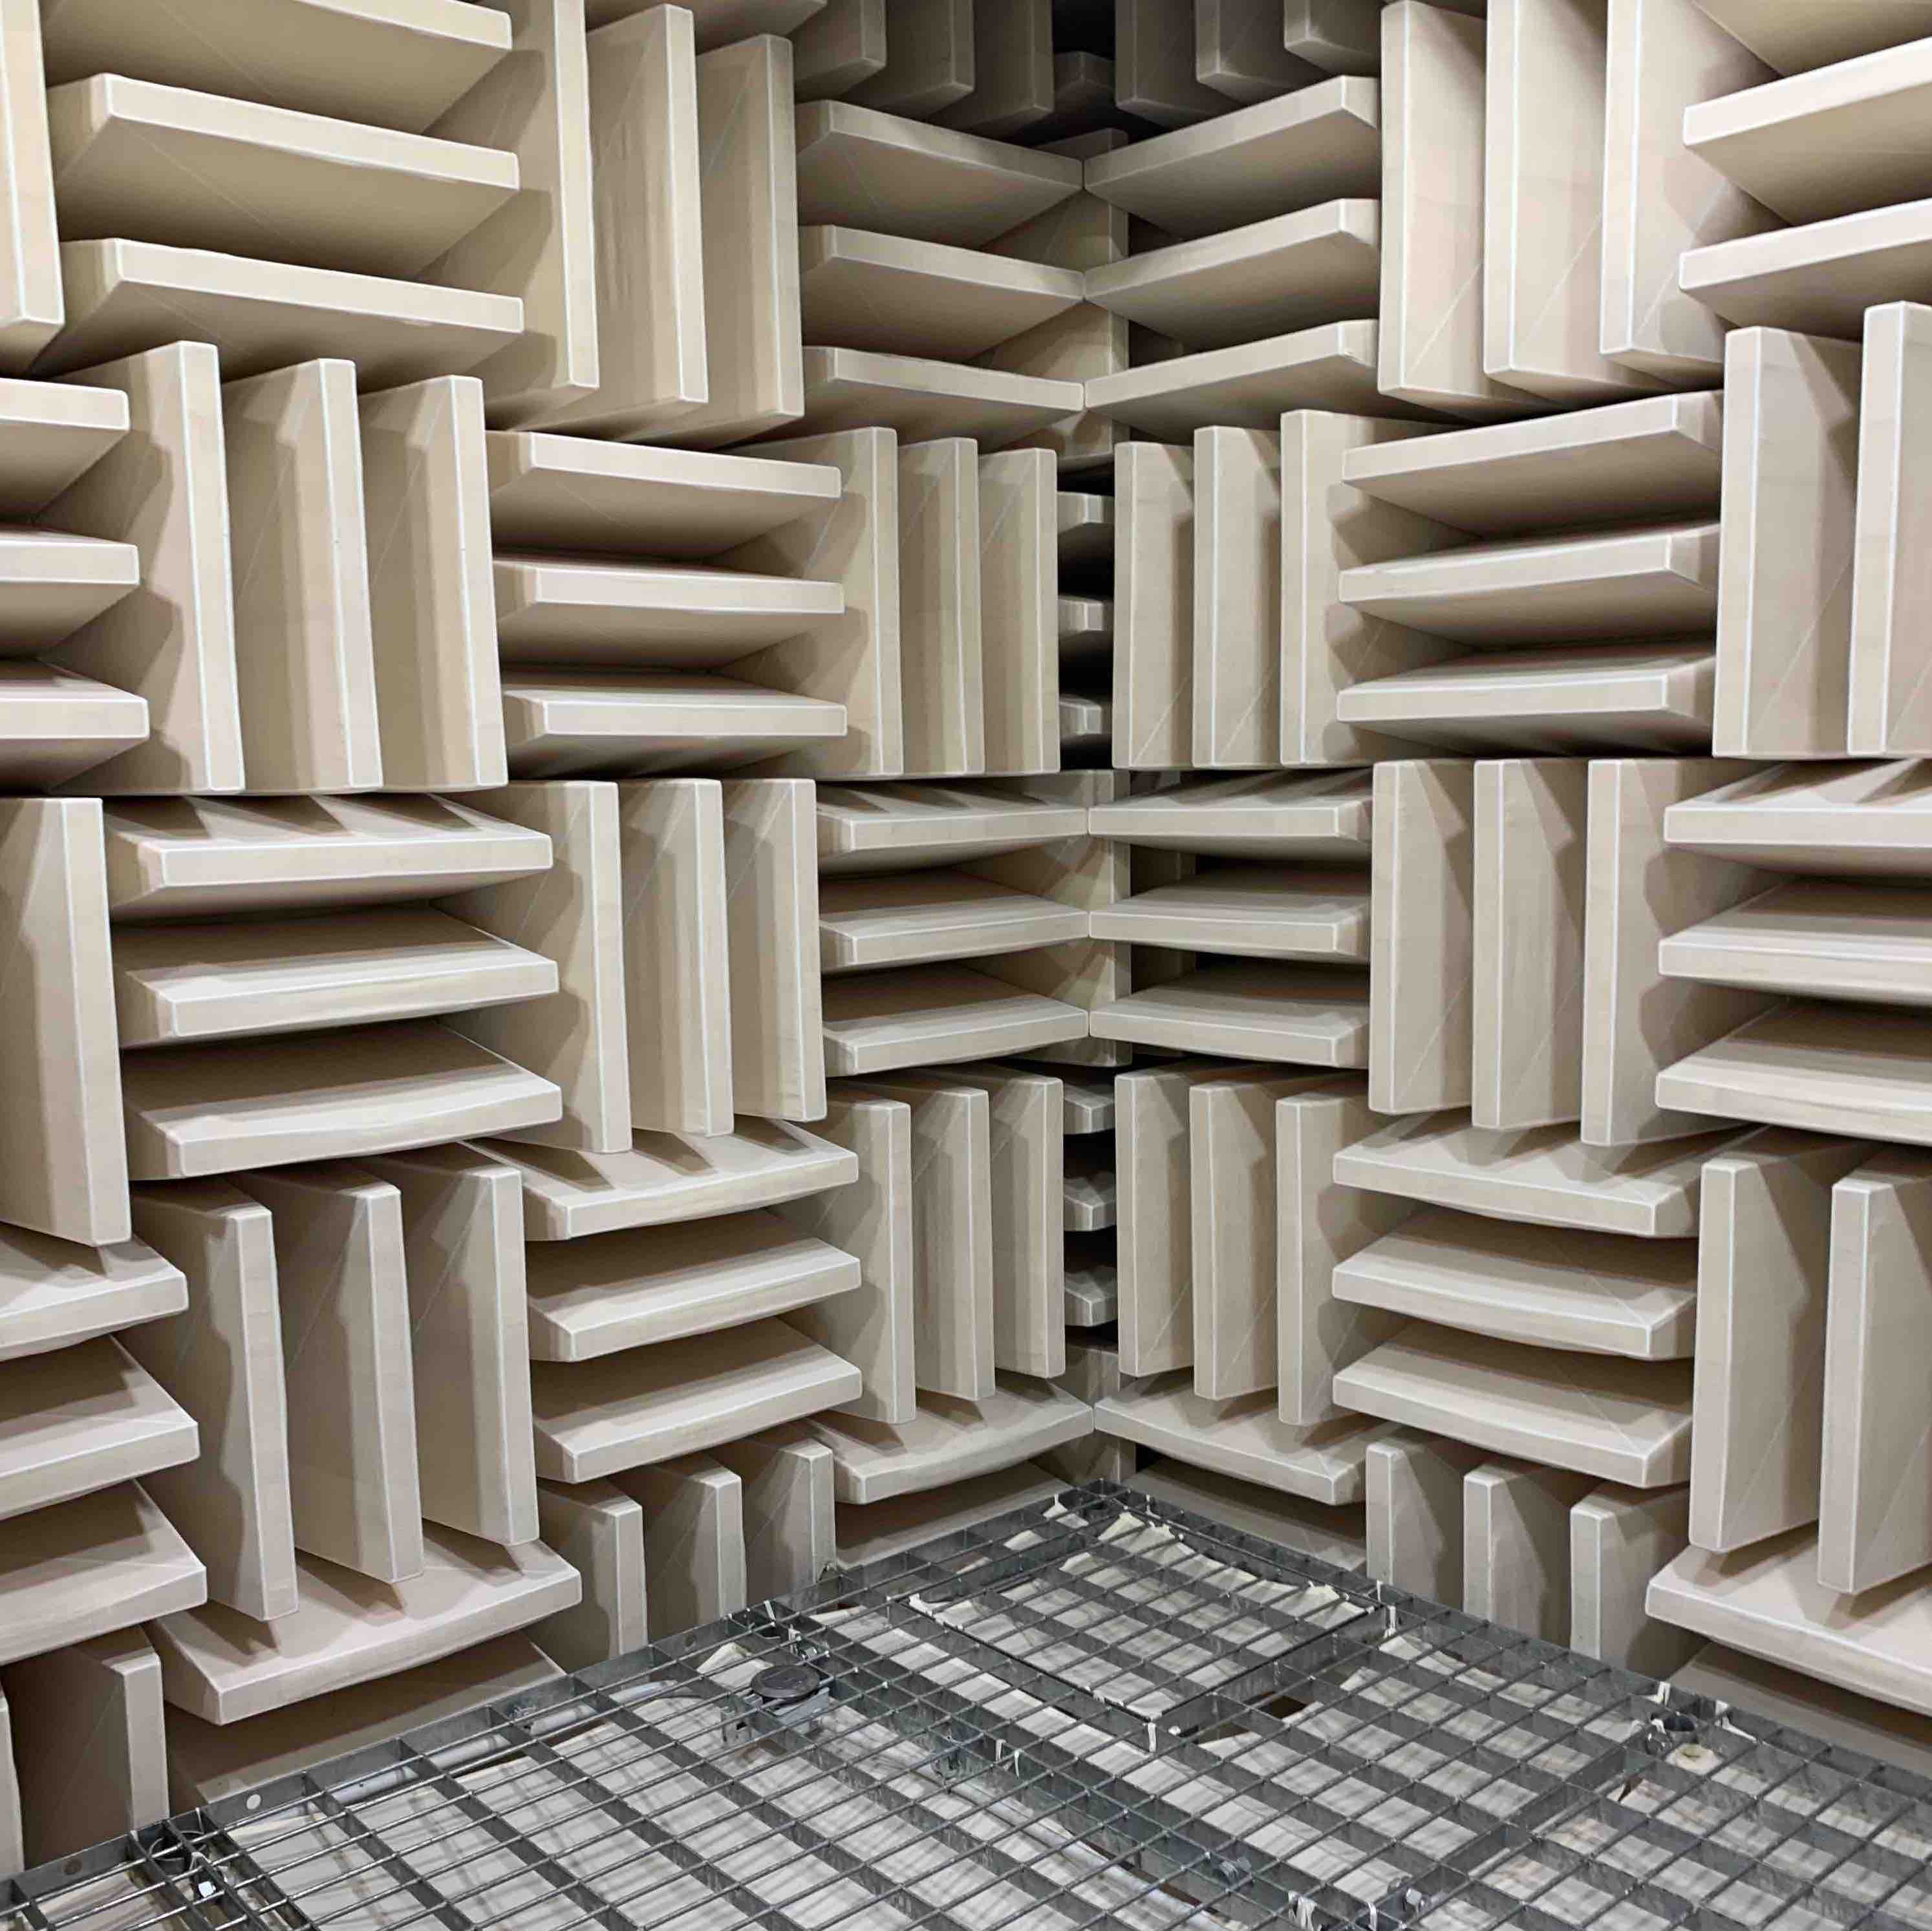
\includegraphics[width=0.6\linewidth]{images/3_anechoic_chamber_ver2.jpg}\label{fig:chamber}}
    \subfigure[Real envitonment (NAIST S1 room)]{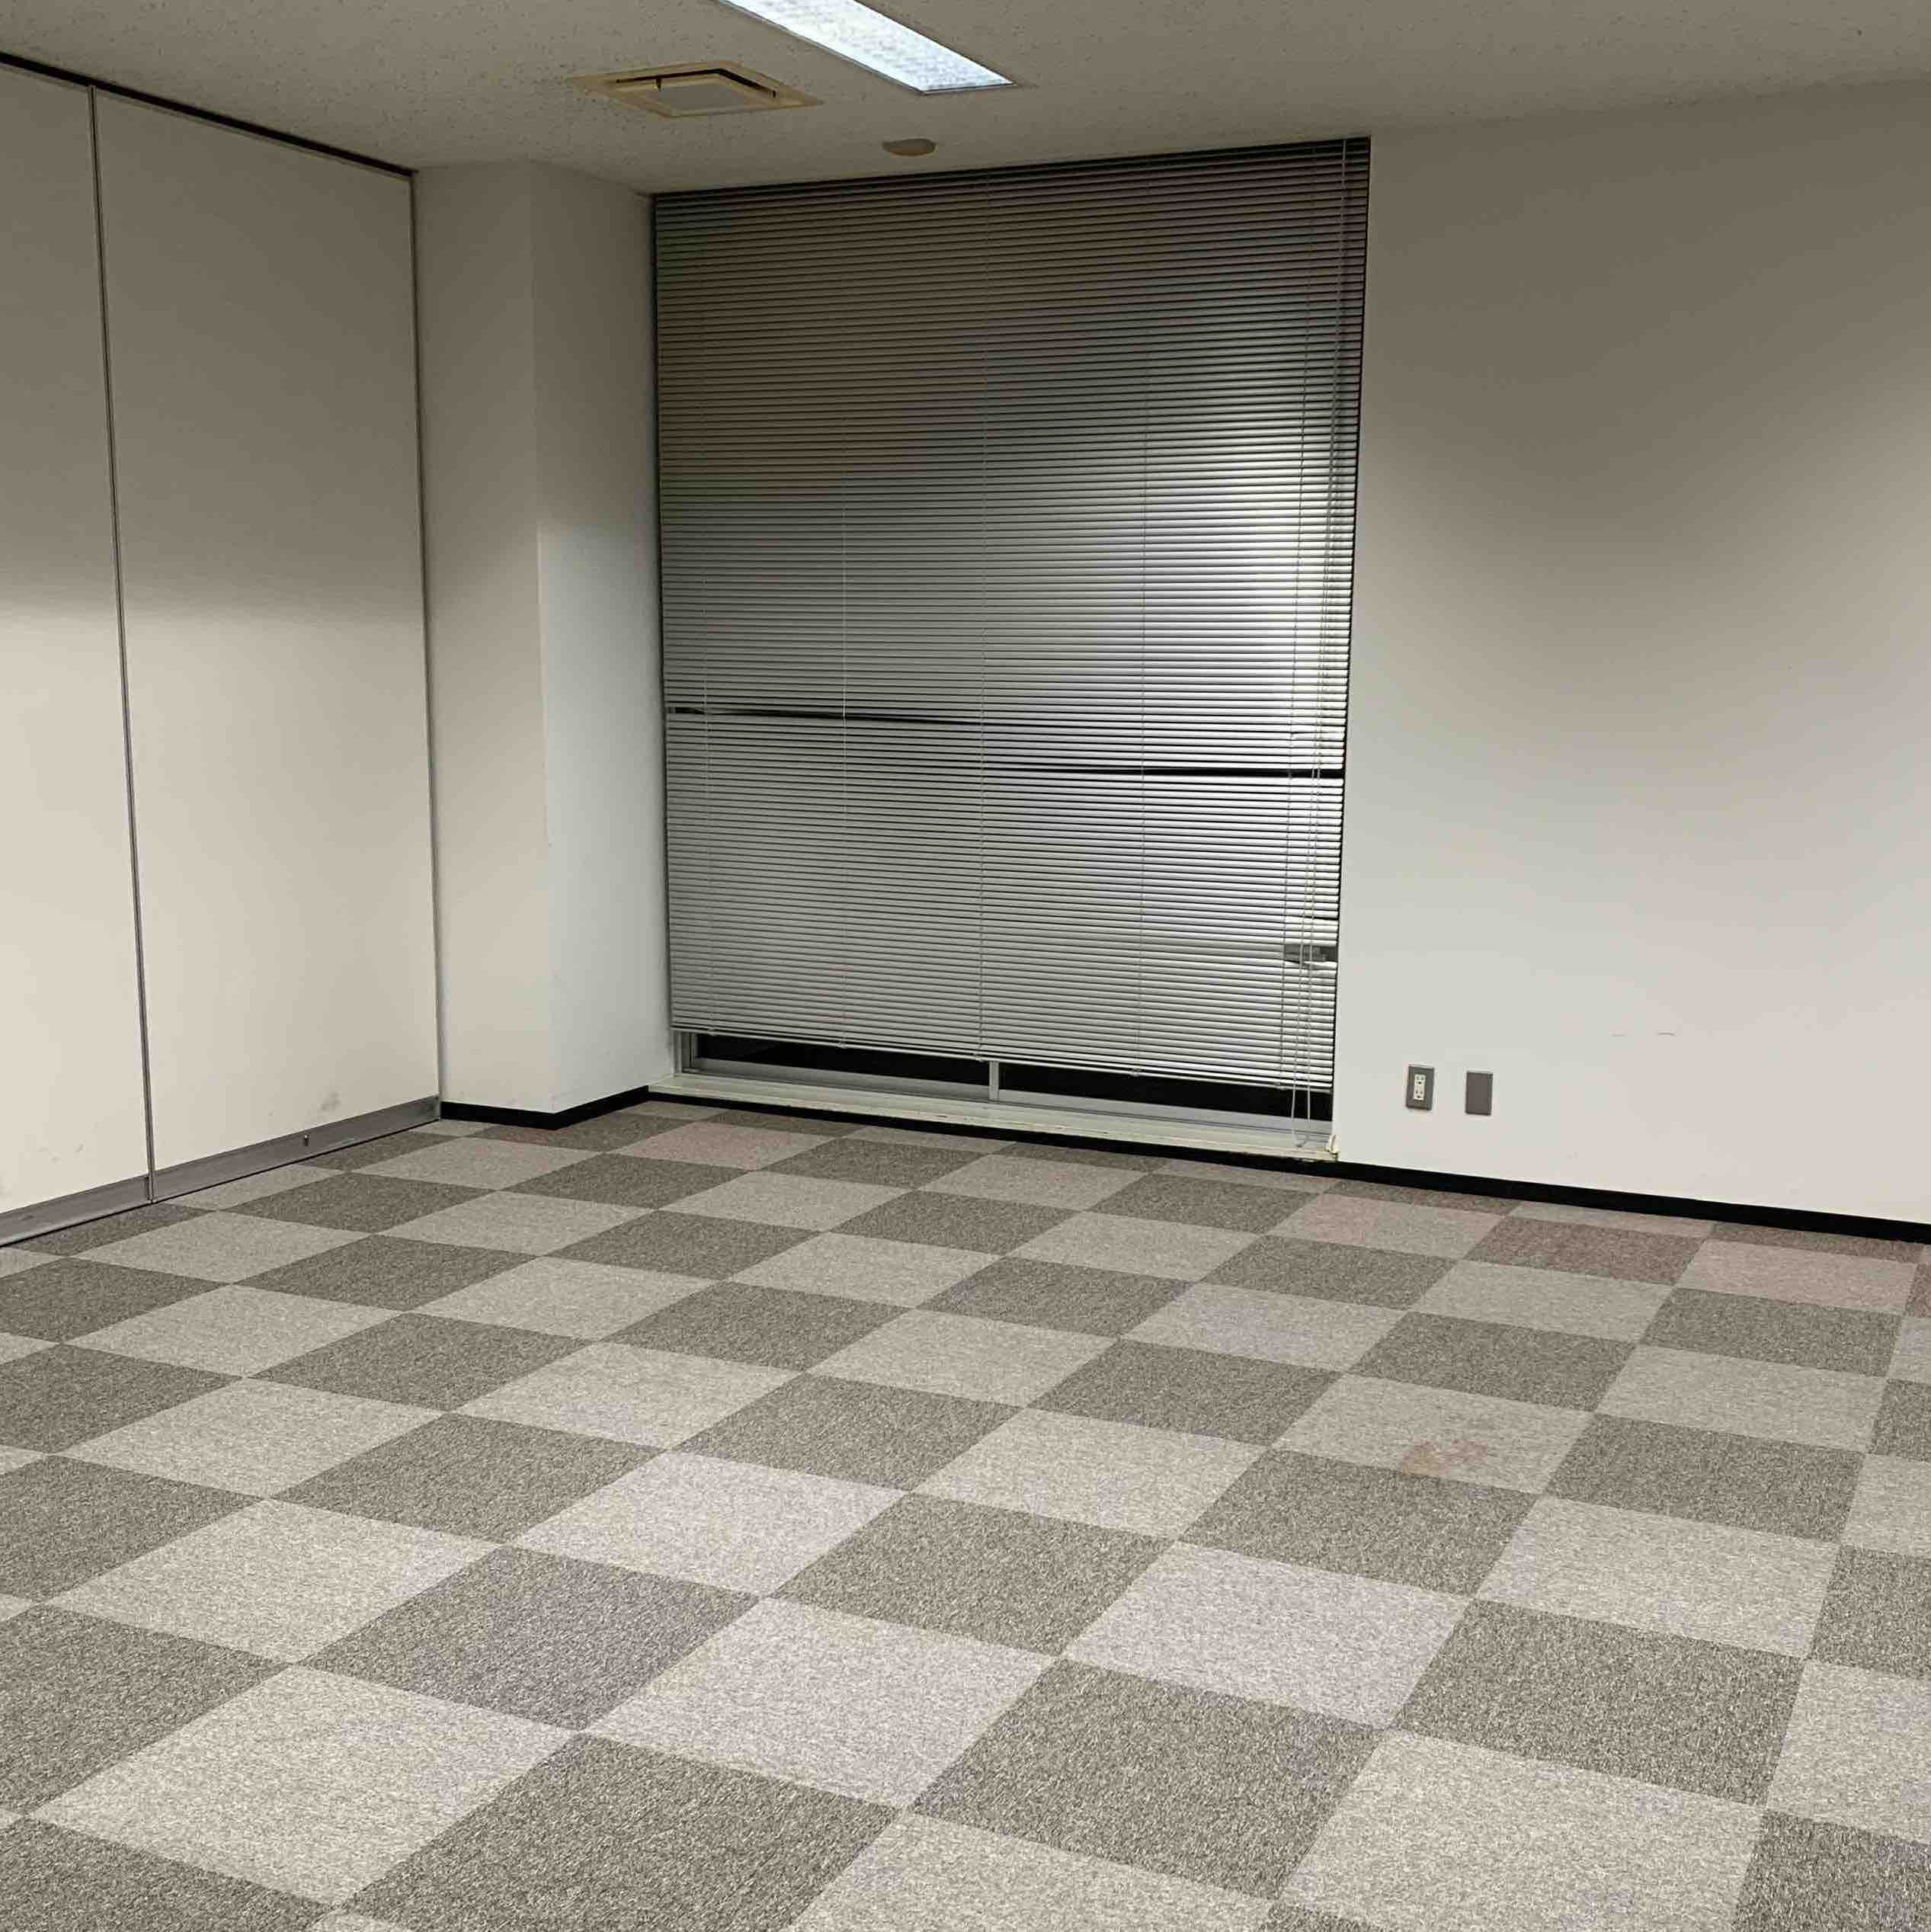
\includegraphics[width=0.6\linewidth]{images/3_naist_s1_ver2.jpg}\label{fig:naist_s1}}
    \caption{Experiment environment}
    \label{fig:exp_photo}
\end{figure}

\clearpage

\subsubsection{実験器具}
実験に用いた道具は以下の通りである。
\begin{itemize}
	\item マイク:Seed社製 Respearker Mic Array V2.0
	\item スピーカ:FPS社製 コンパクトオーディオスピーカー(SW5500-SS)
    \item 回転台:シグマ光機社製 小型回転ステージ(OSMS-60YAW)
    \item 平面:ガラス板(横32×縦23)
\end{itemize}
マイクは4つのマイクロホンを搭載しあたマイクロホンアレイを用いた。理由としては、Beamforming技術を用いることで音源の到来方向を制限するためである。今回、スピーカをマイクと対象平面とは180[deg]反対側に配置した。これにより、Beamformingを用いることで、スピーカ側180[deg]の音源を取らないように制限することができる。これにより、直接音を弱め、反射音を強めることができると考えた。

スピーカは平面波スピーカを使用している。普段、音は近傍界、遠方界によって波の形状が変化する。近傍界では球面波、遠方界では平面波となる。今回の手法を用いる場合、音源の入射方向が一意に決まる必要があるため、平面波を用いることが必要である。そのため、平面波を出力の時点で出すことができるスピーカを用いることでこの問題を解決した

回転台は平面の方位角との収録音の関係を取得するために使用する。本実験では、1[deg]ごとに変化させた実験データ収録する。。今回使用した回転台は最小単位が0.0001[deg]の精度で回転させることができる。そのため、今回欲しい平面の方位角を1[deg]ごとに-50[deg] $\sim$ 50[deg]を取るには十分だと考えている。また、停止時の振動と移動時の雑音も少ないため、今回のような音を使った実験を行うのに最適だと考えた。
さらに、本実験ではバックラッシュ誤差が少しでも出ないように1[deg]を連続で変化させるのではなく、10[deg]ずつ変化させ、データを集めた。

平面にはガラス板を用いた。理由としては2点ある。1点目は、ガラスは表面が非常になめらかであるため、拡散反射率がより理論値に近づくと考えた点である。2点目はカメラでの認識が難しく音波を使うことの有用性が考えられる点である。

\begin{figure}[ht]
    \centering
    \subfigure[Respeaker Microphone Array V2.0]{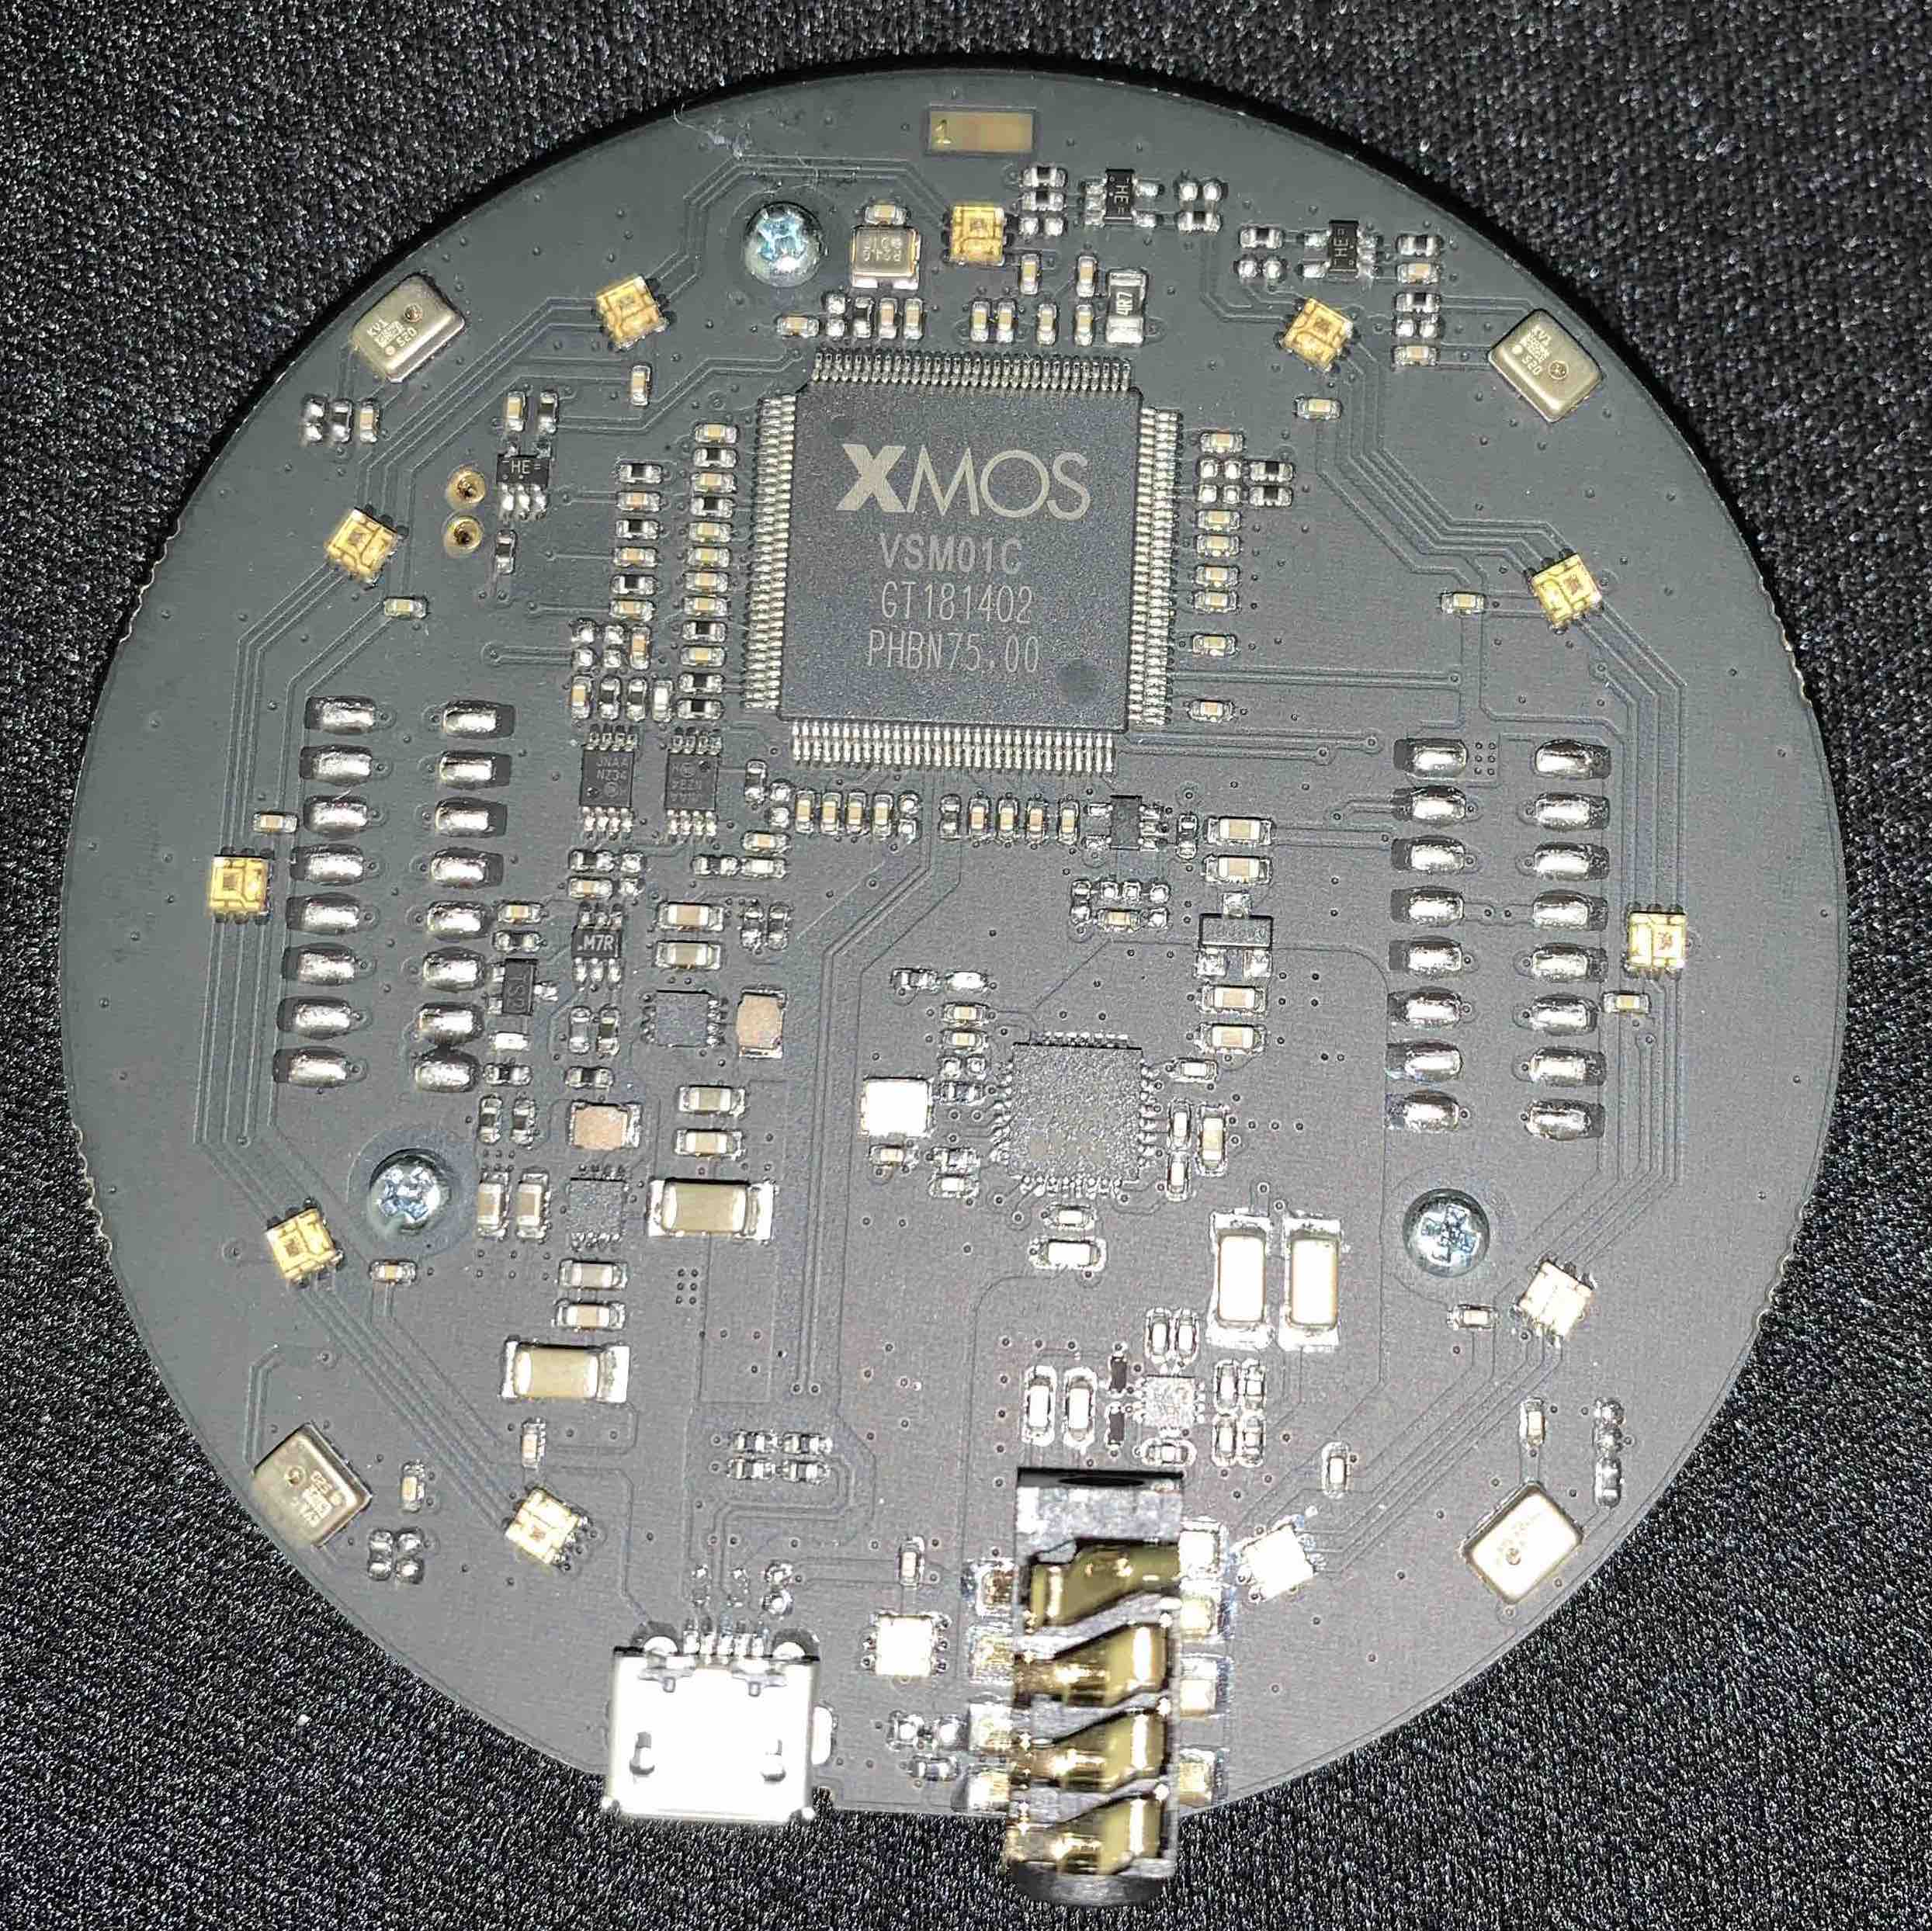
\includegraphics[width=0.4\linewidth]{images/3_respeaker.jpg}}
    \label{fig:respeaker_mic}
    \subfigure[SW5500-SS]{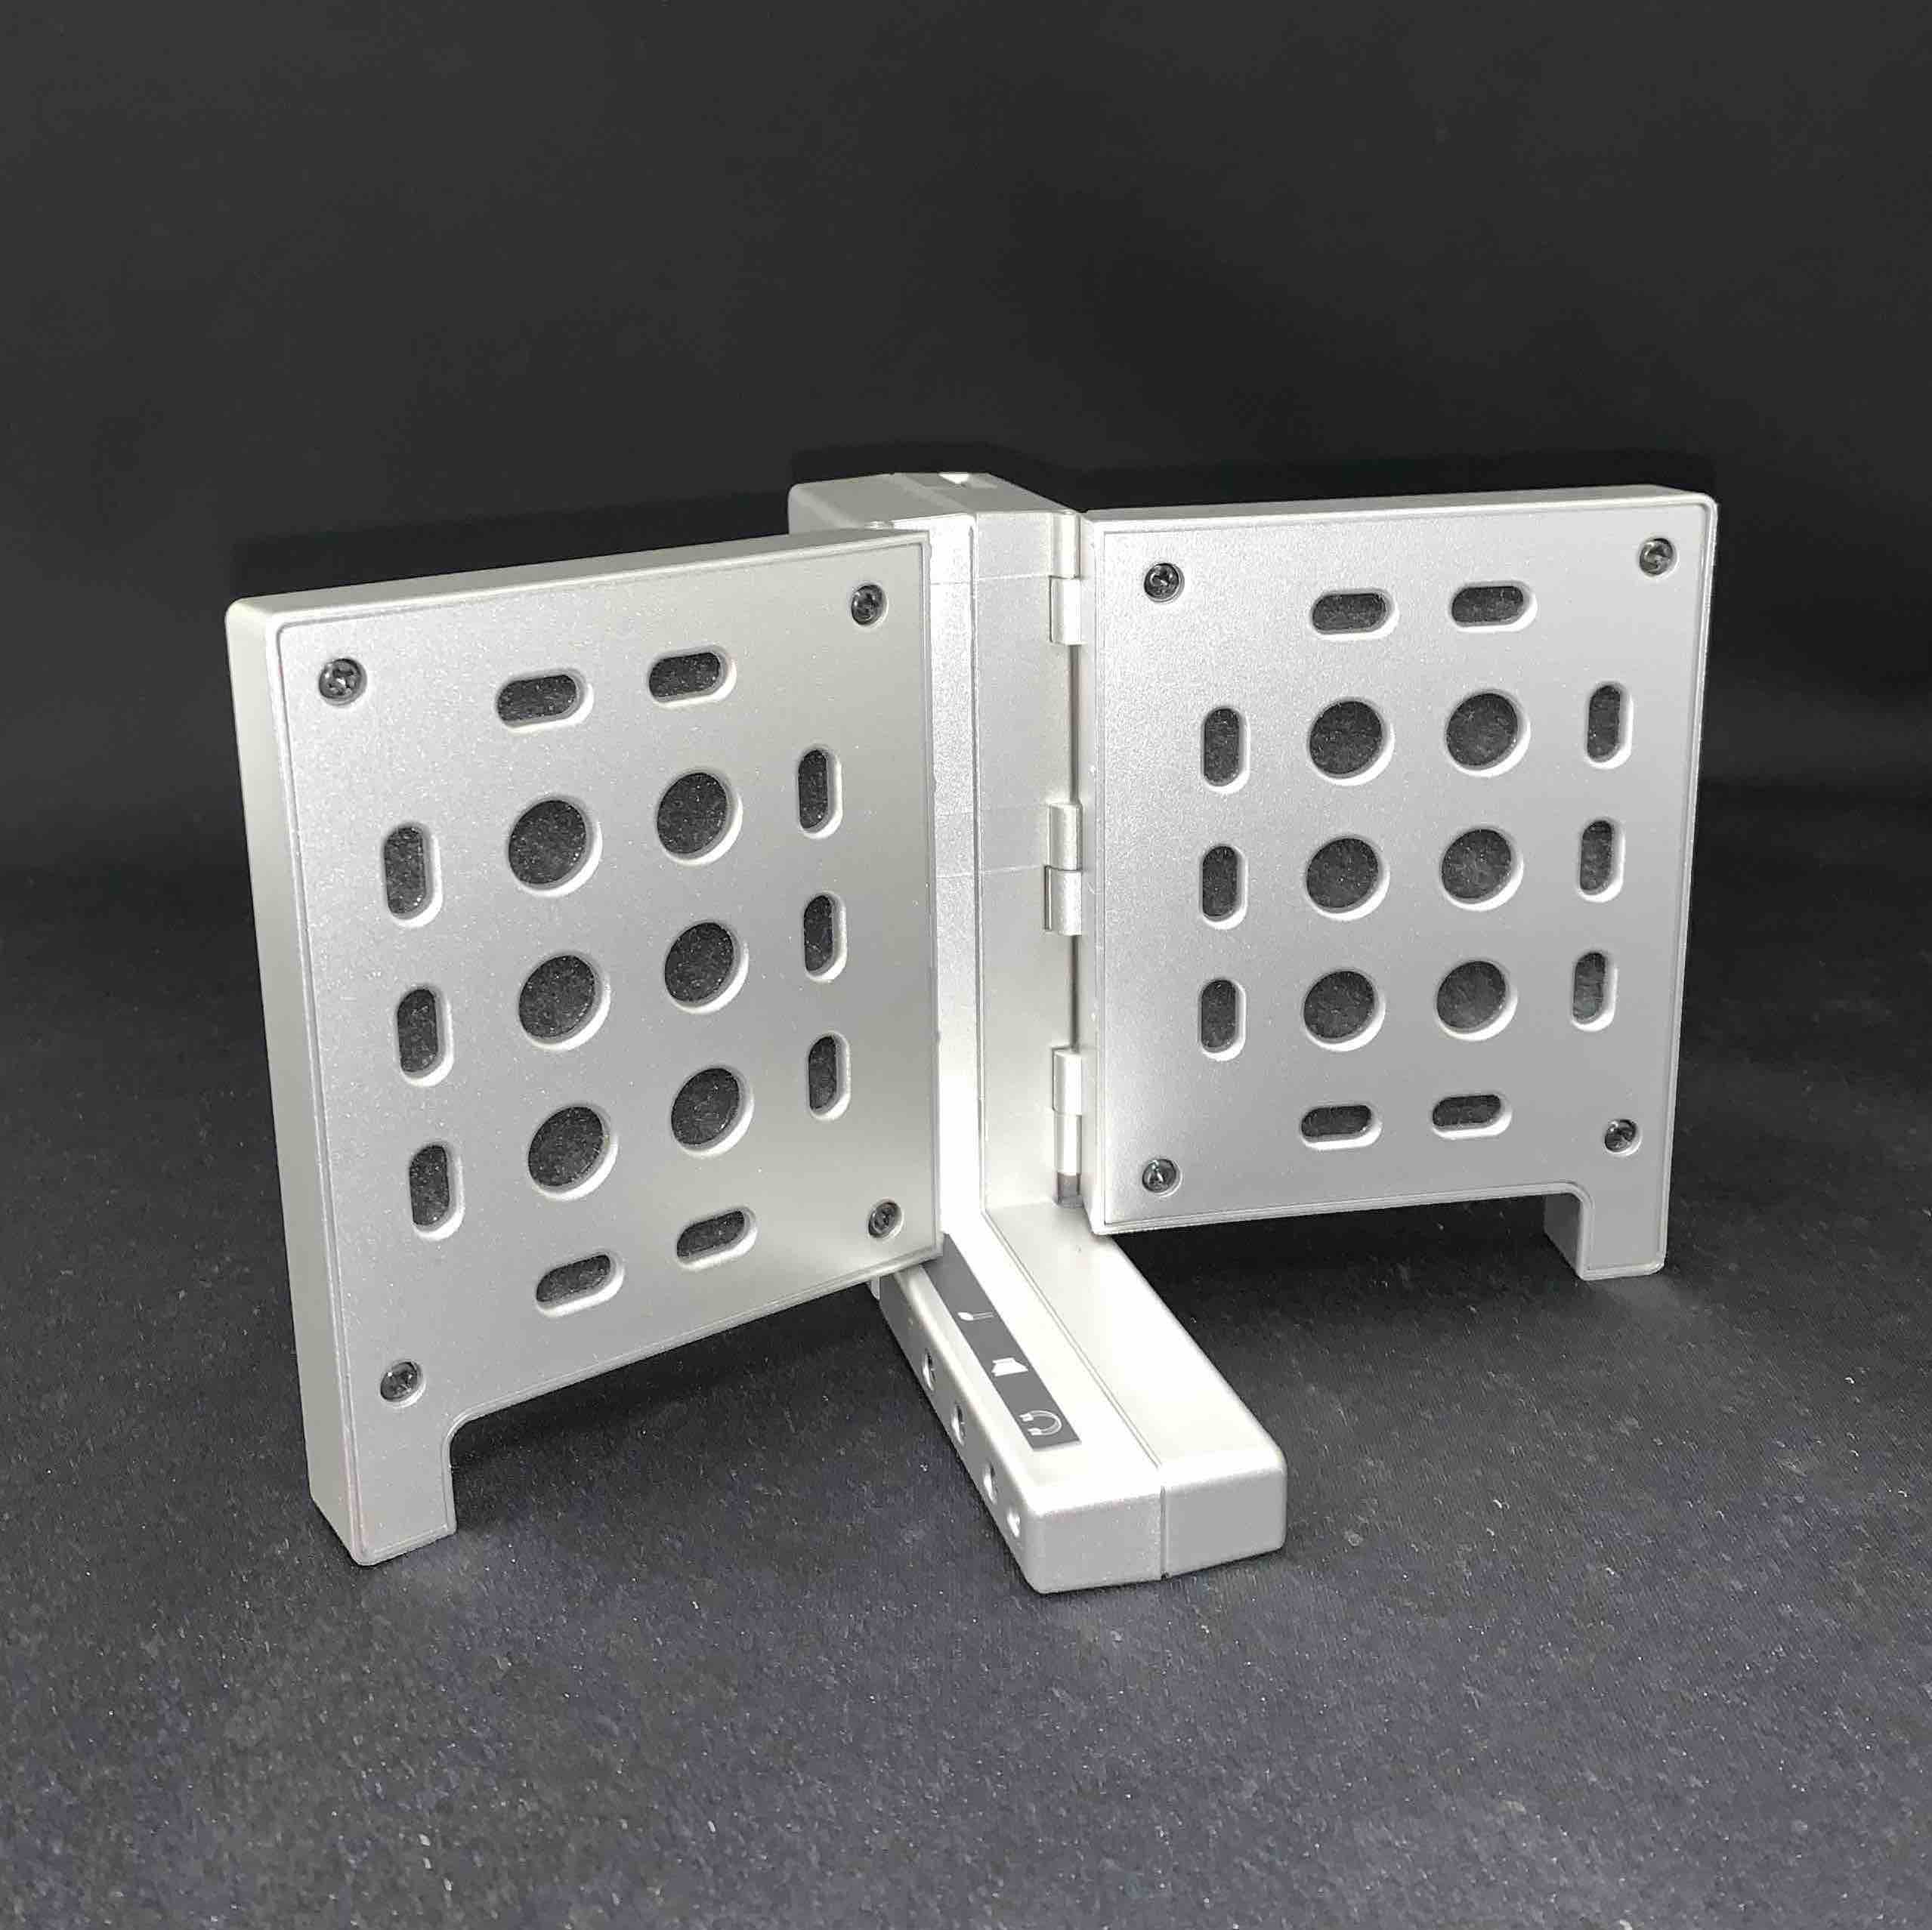
\includegraphics[width=0.4\linewidth]{images/3_plane_speaker.jpg}}
    \label{fig:plane_speaker}
    \subfigure[OSMS-60YAW]{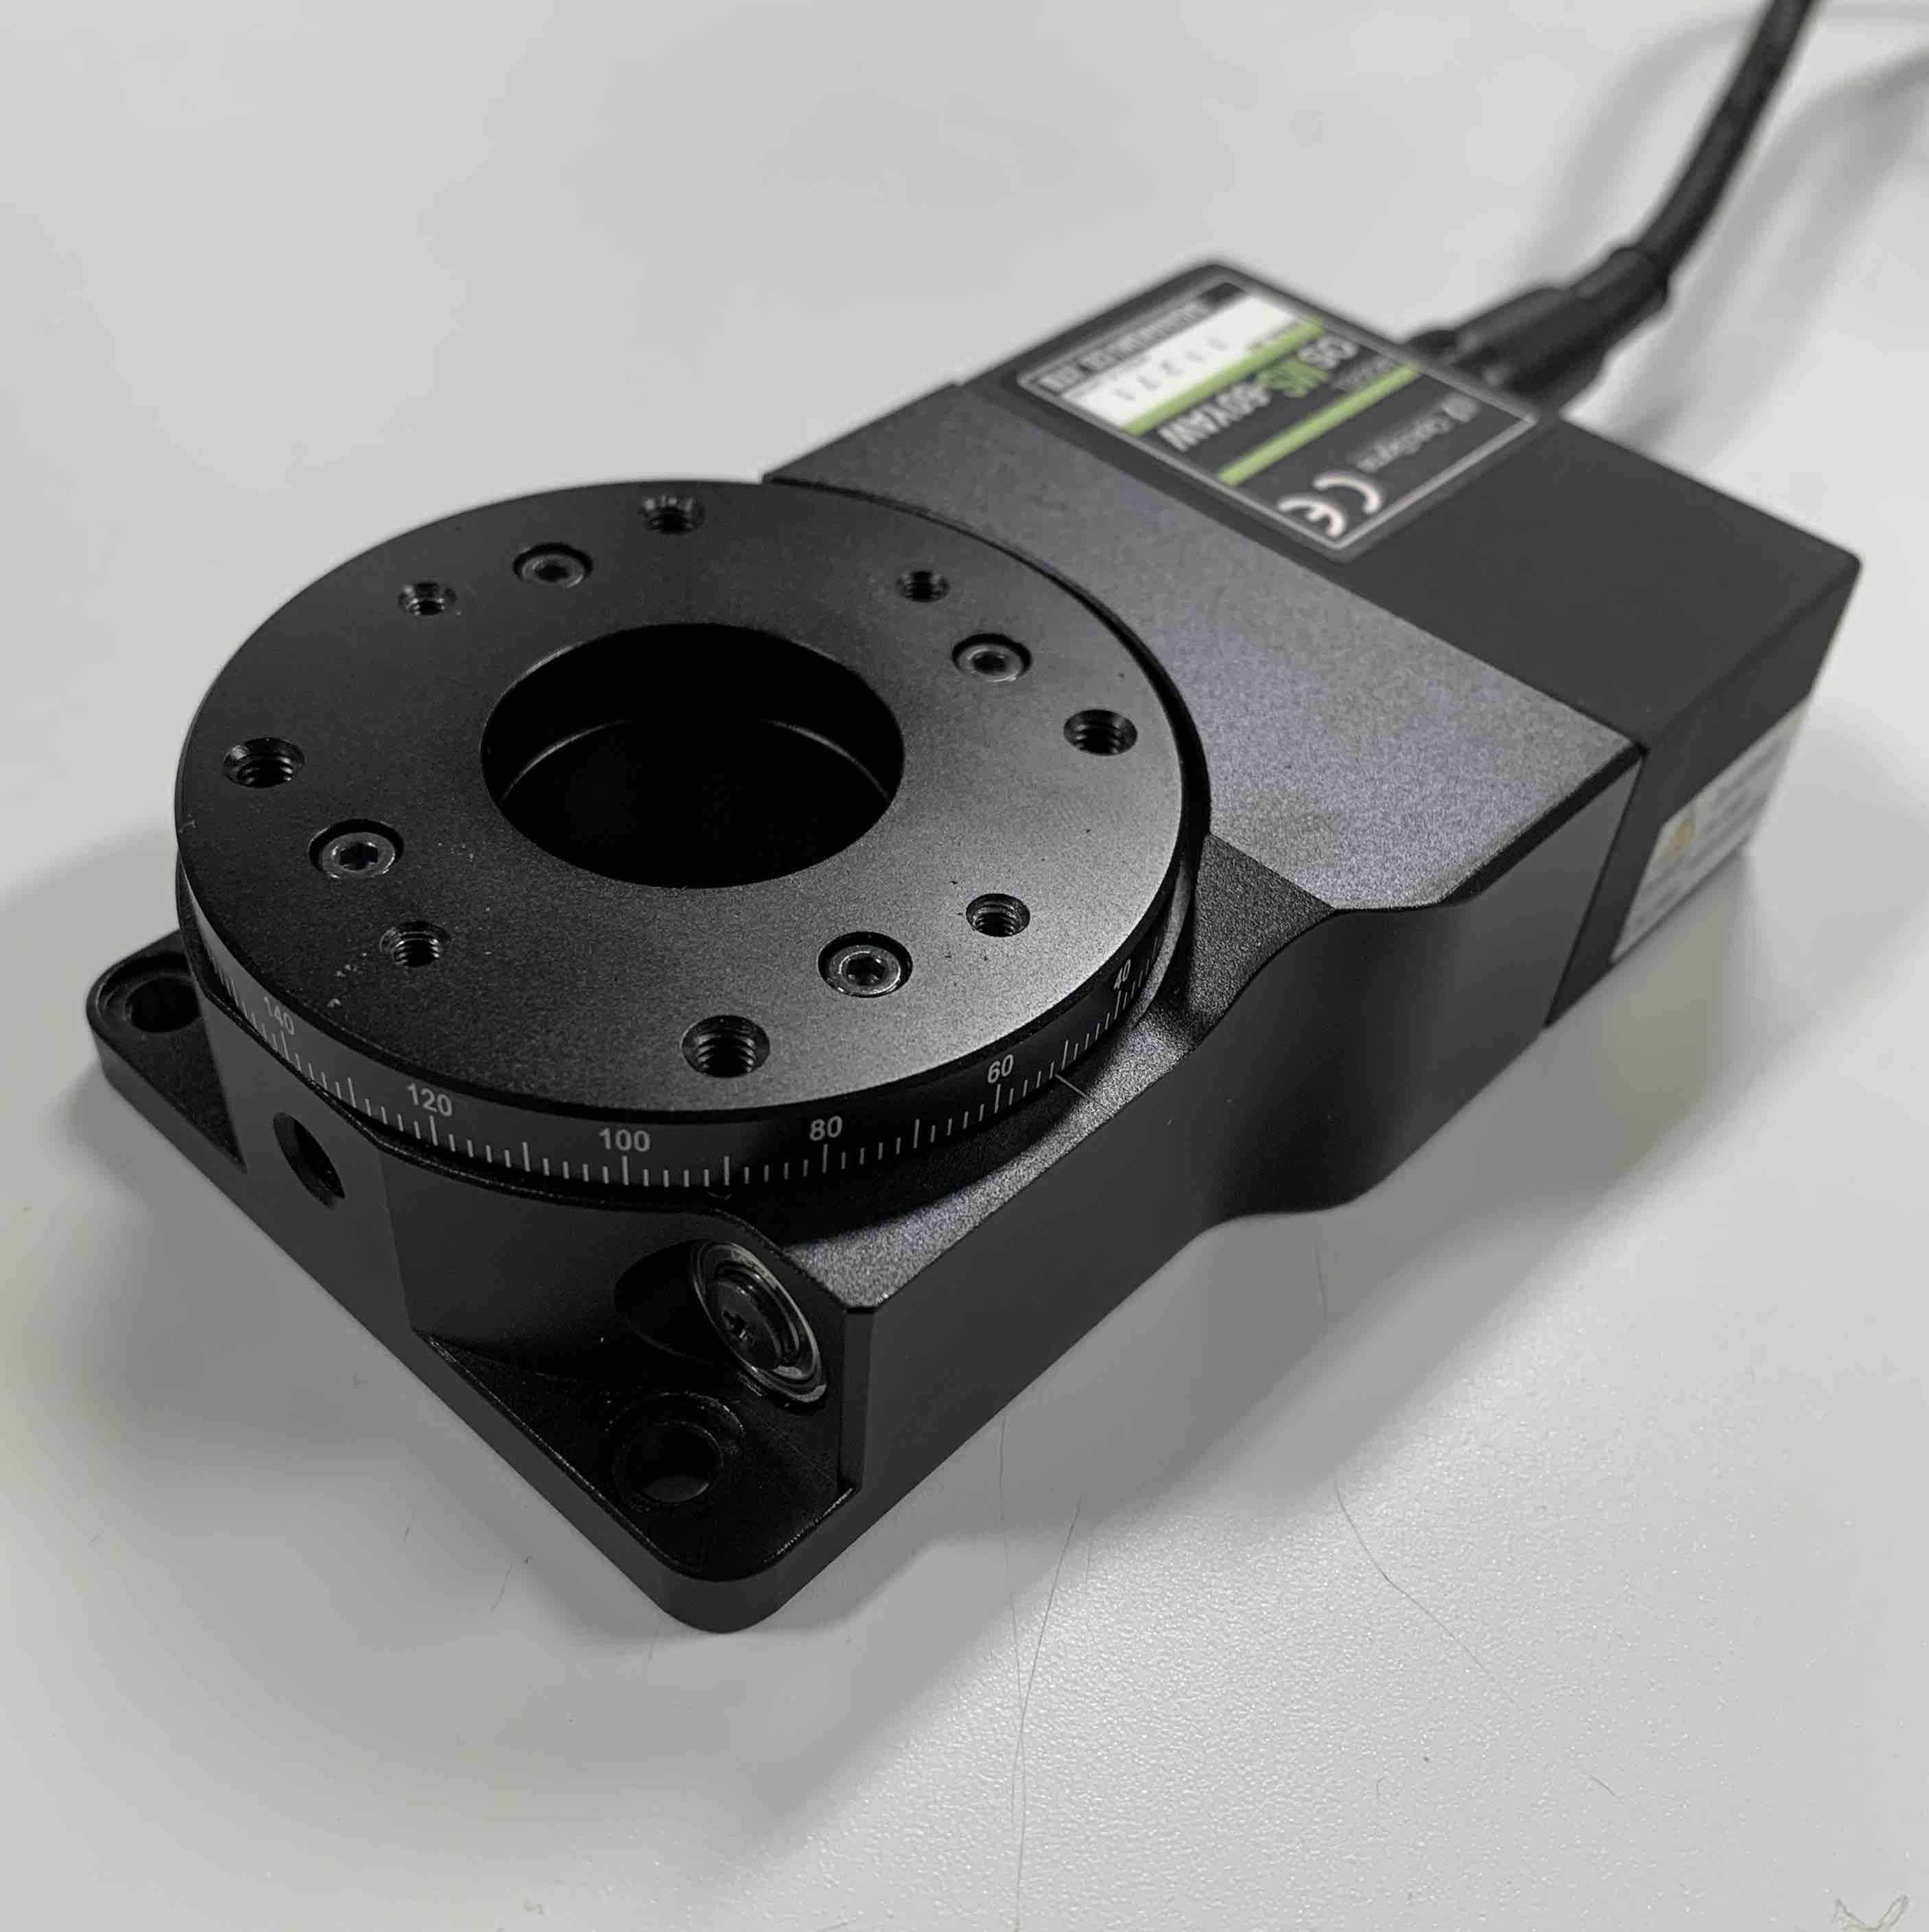
\includegraphics[width=0.4\linewidth]{images/3_turntable.jpg}}
    \label{fig:turn_table}
    \subfigure[Mirro plate (h: 23, l: 32)]{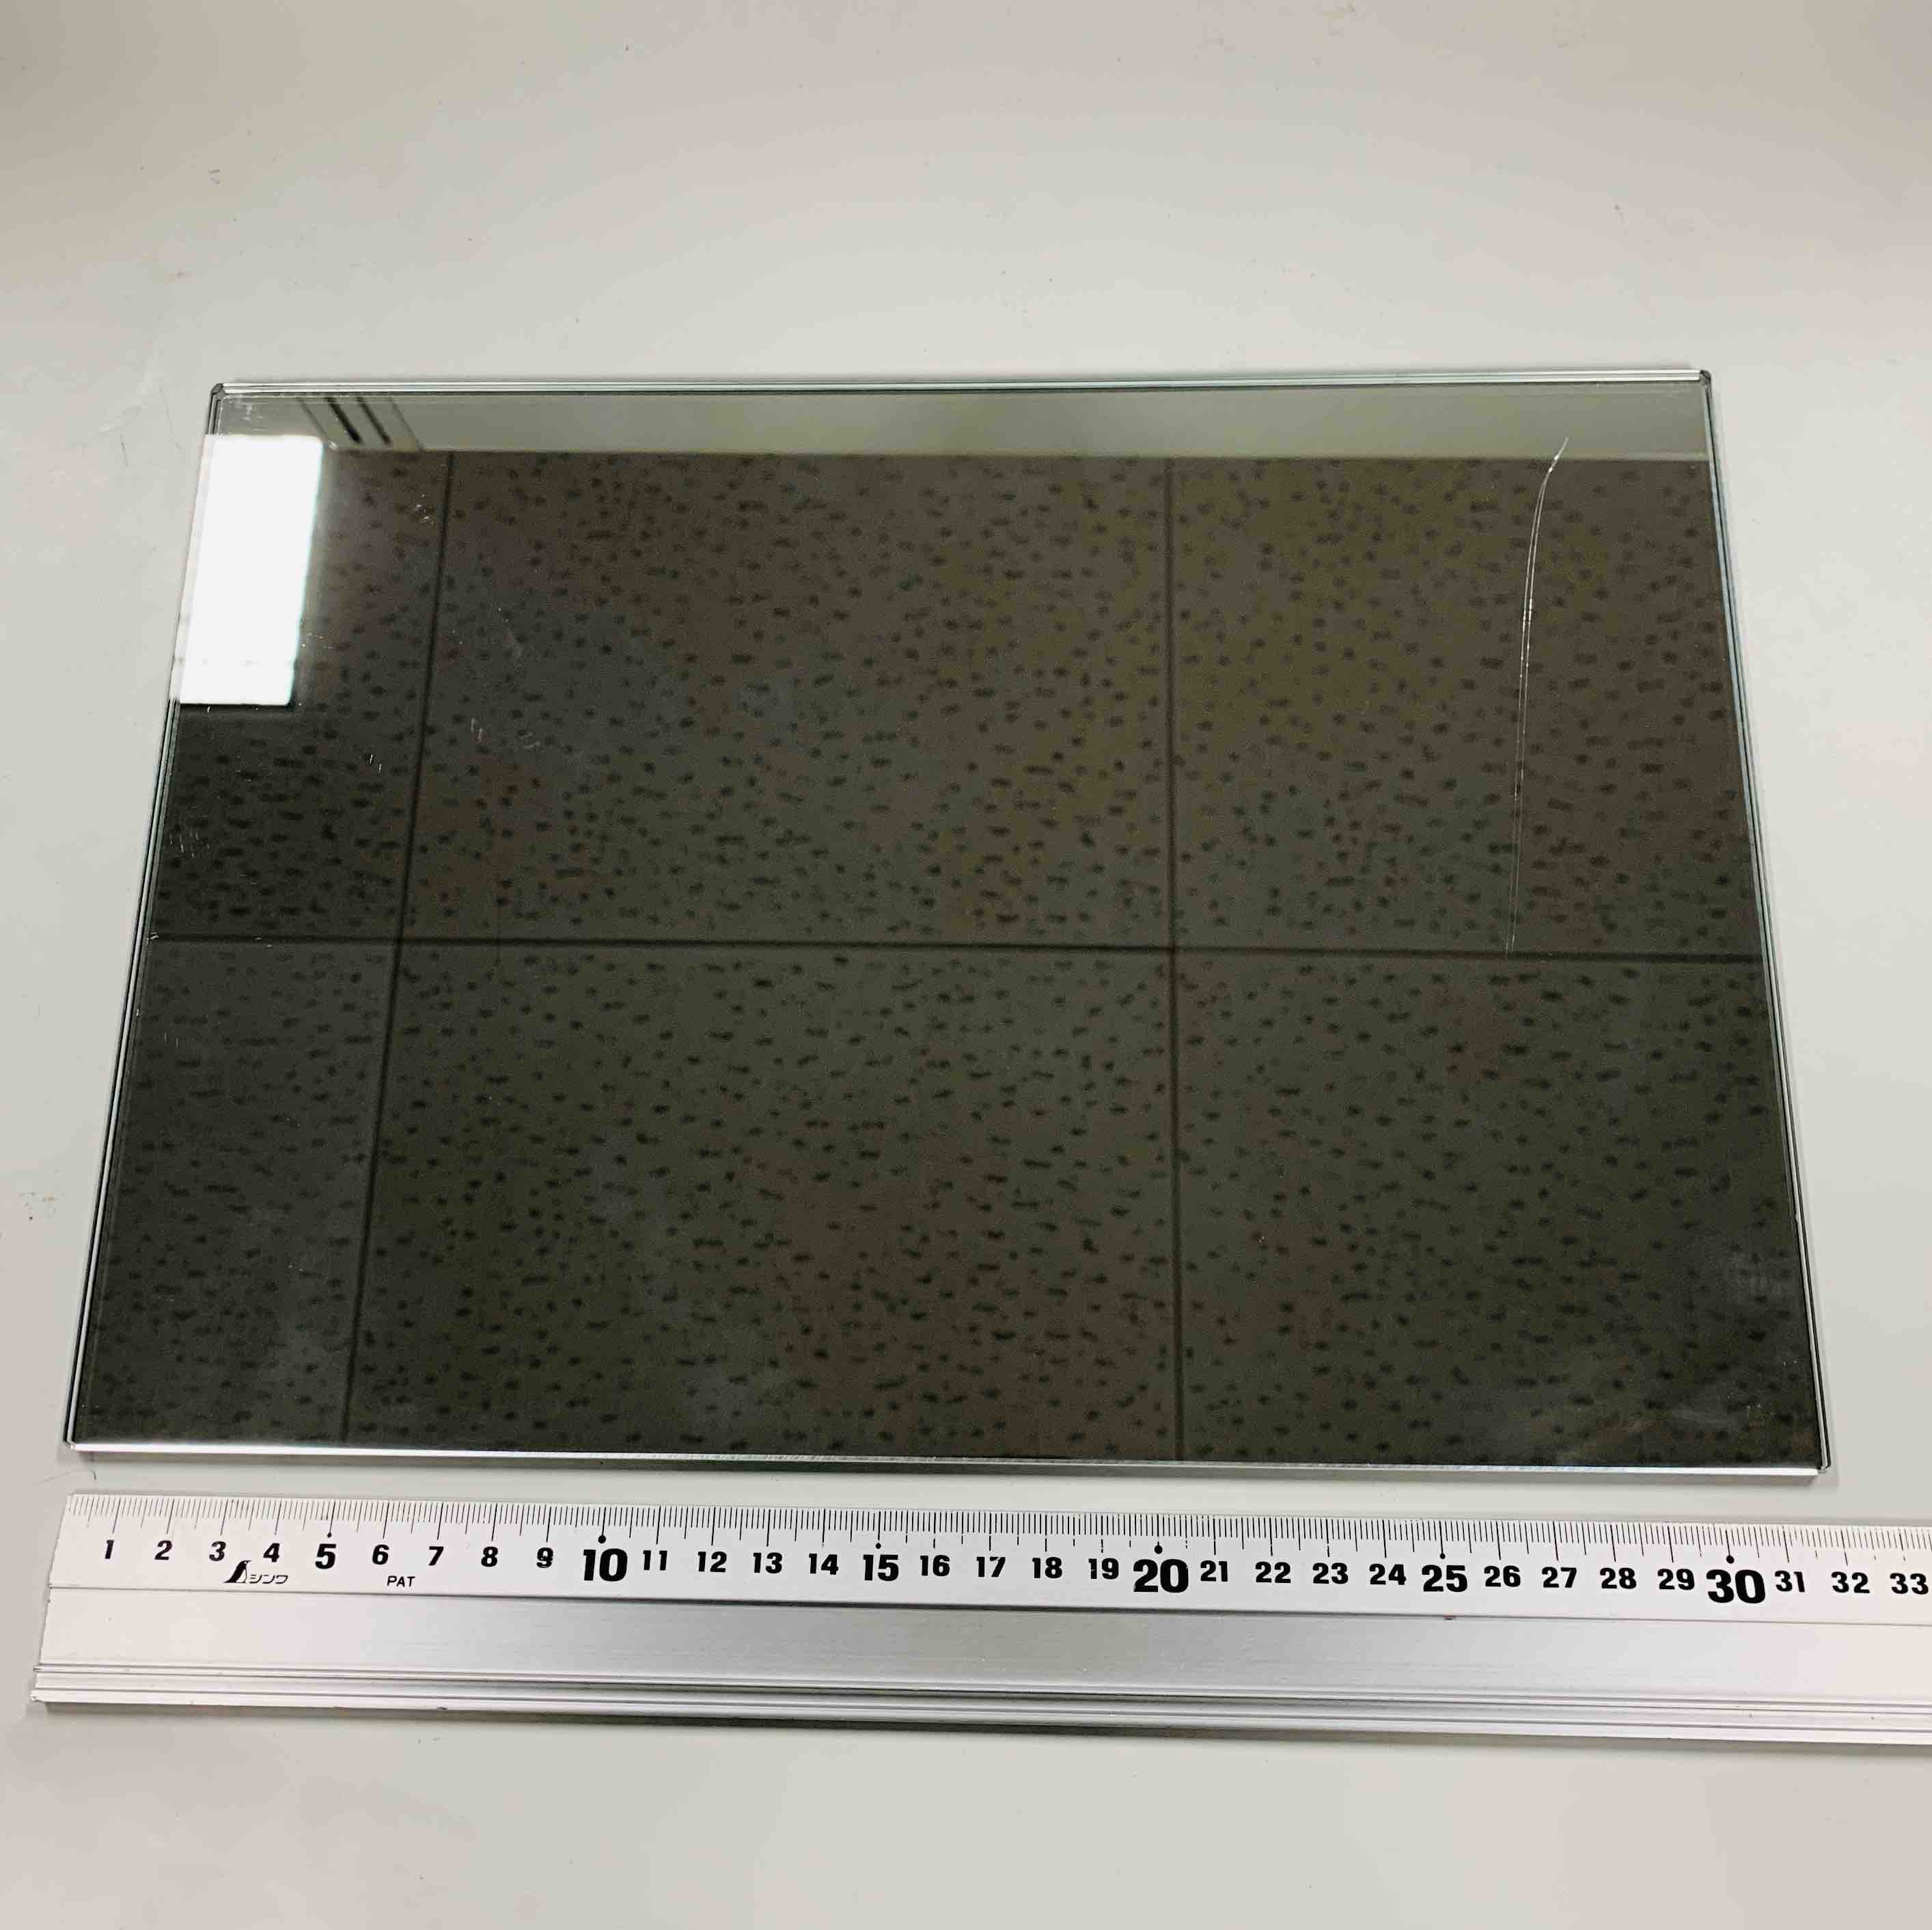
\includegraphics[width=0.4\linewidth]{images/3_mirror_ver1.jpg}}
    \label{fig:mirror_ver1}
    \caption{Experiment equipment images}
    \label{fig:exp_equipment}
\end{figure}

\clearpage

\subsubsection{実験方法}
スピーカからUp-TSP信号を出力し、その反射音ををマイクロホンアレイにより取得する。今回、Up-TSP信号を使用した点には2点ある。1点目は全周波数の情報を持っているためである。今回、周波数領域の情報が重要である。そのため、全周波数を持つTSP信号を用いることを考えた。2点目はTSP信号の本来の使い方であるインパルス応答を見ることができ、伝達関数を作成可能という点である。この伝達関数を参考にすることで、モデル作成に関して有益な情報を見つけることができないかとかと考えた。さらに、その中でもUp-TSP信号を採用した理由としては、周波数特性に対して外乱が少ないためである。[参考文献]

実験の簡略図を\figref{exp_pos_para}, 実験をした際のパラメータを\tabref{exp_para}, 
実験の様子を\figref{exp_env}に示す。

\begin{figure}[ht]
  \begin{center}
  \vspace{1zh}
    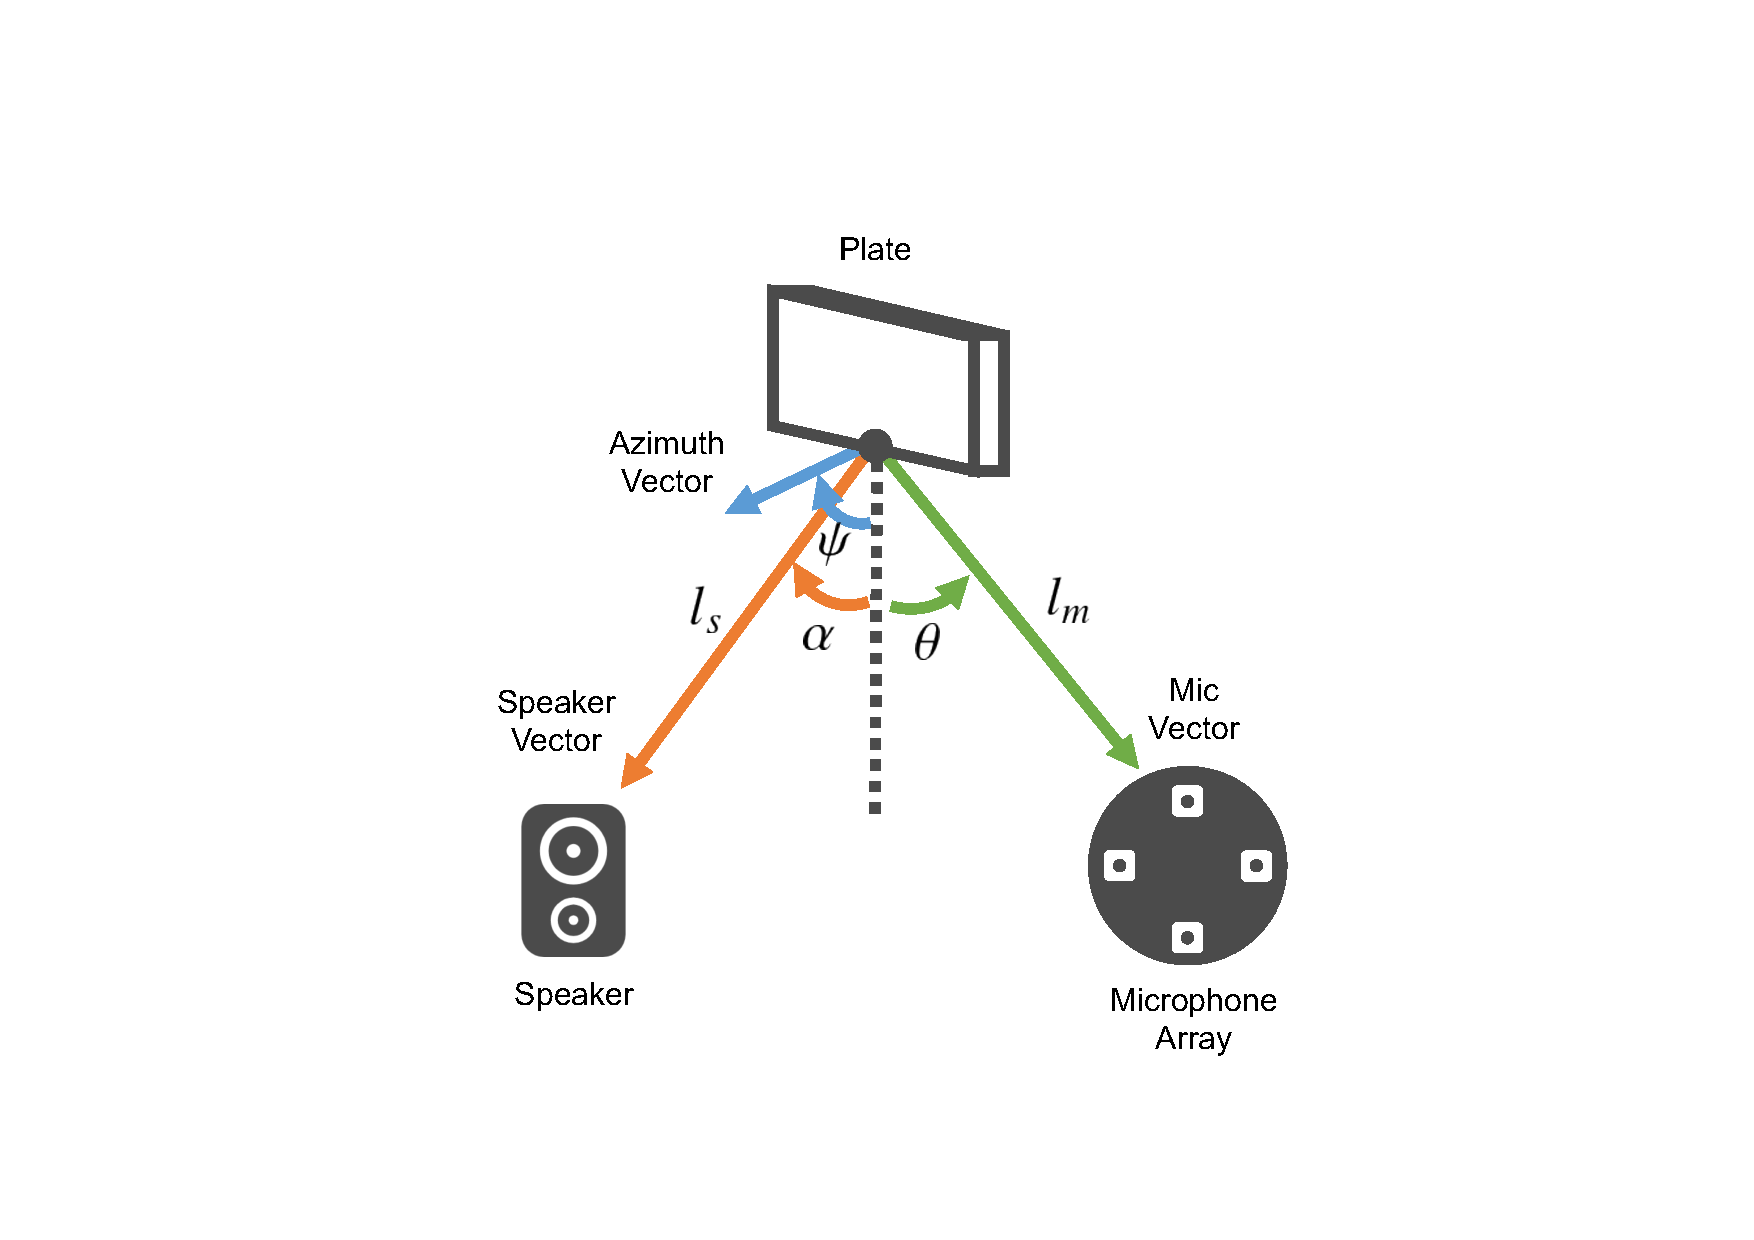
\includegraphics[width=0.55\linewidth]{images/3_exp_pos_para.pdf}  
  \end{center}
  \caption{Position and parametor for experiment checking model}
  \label{fig:exp_pos_para}
\end{figure}

\begin{table}[ht]
    \centering
    \caption{Value of parametar for experiment checking model}
    \begin{tabular}{c|c}\hline
        Parametor & Value \\ \hline\hline
        $\alpha [\mathrm{deg}]$ & 0 \\ \hline
        $\psi [\mathrm{deg}]$ & $-50 \sim 50$ (per 1 [deg])\\ \hline
        $\theta [\mathrm{deg}]$ & 0 \\ \hline
        $l_m [\mathrm{m}]$ & 0.2 \\ \hline
        $l_s [\mathrm{m}]$ & 0.4 \\ \hline
        % $\rho$ & 0.9 \\\hline
    \end{tabular}
    \label{tab:exp_para}
\end{table}

\begin{figure}[ht]
  \begin{center}
  \vspace{1zh}
    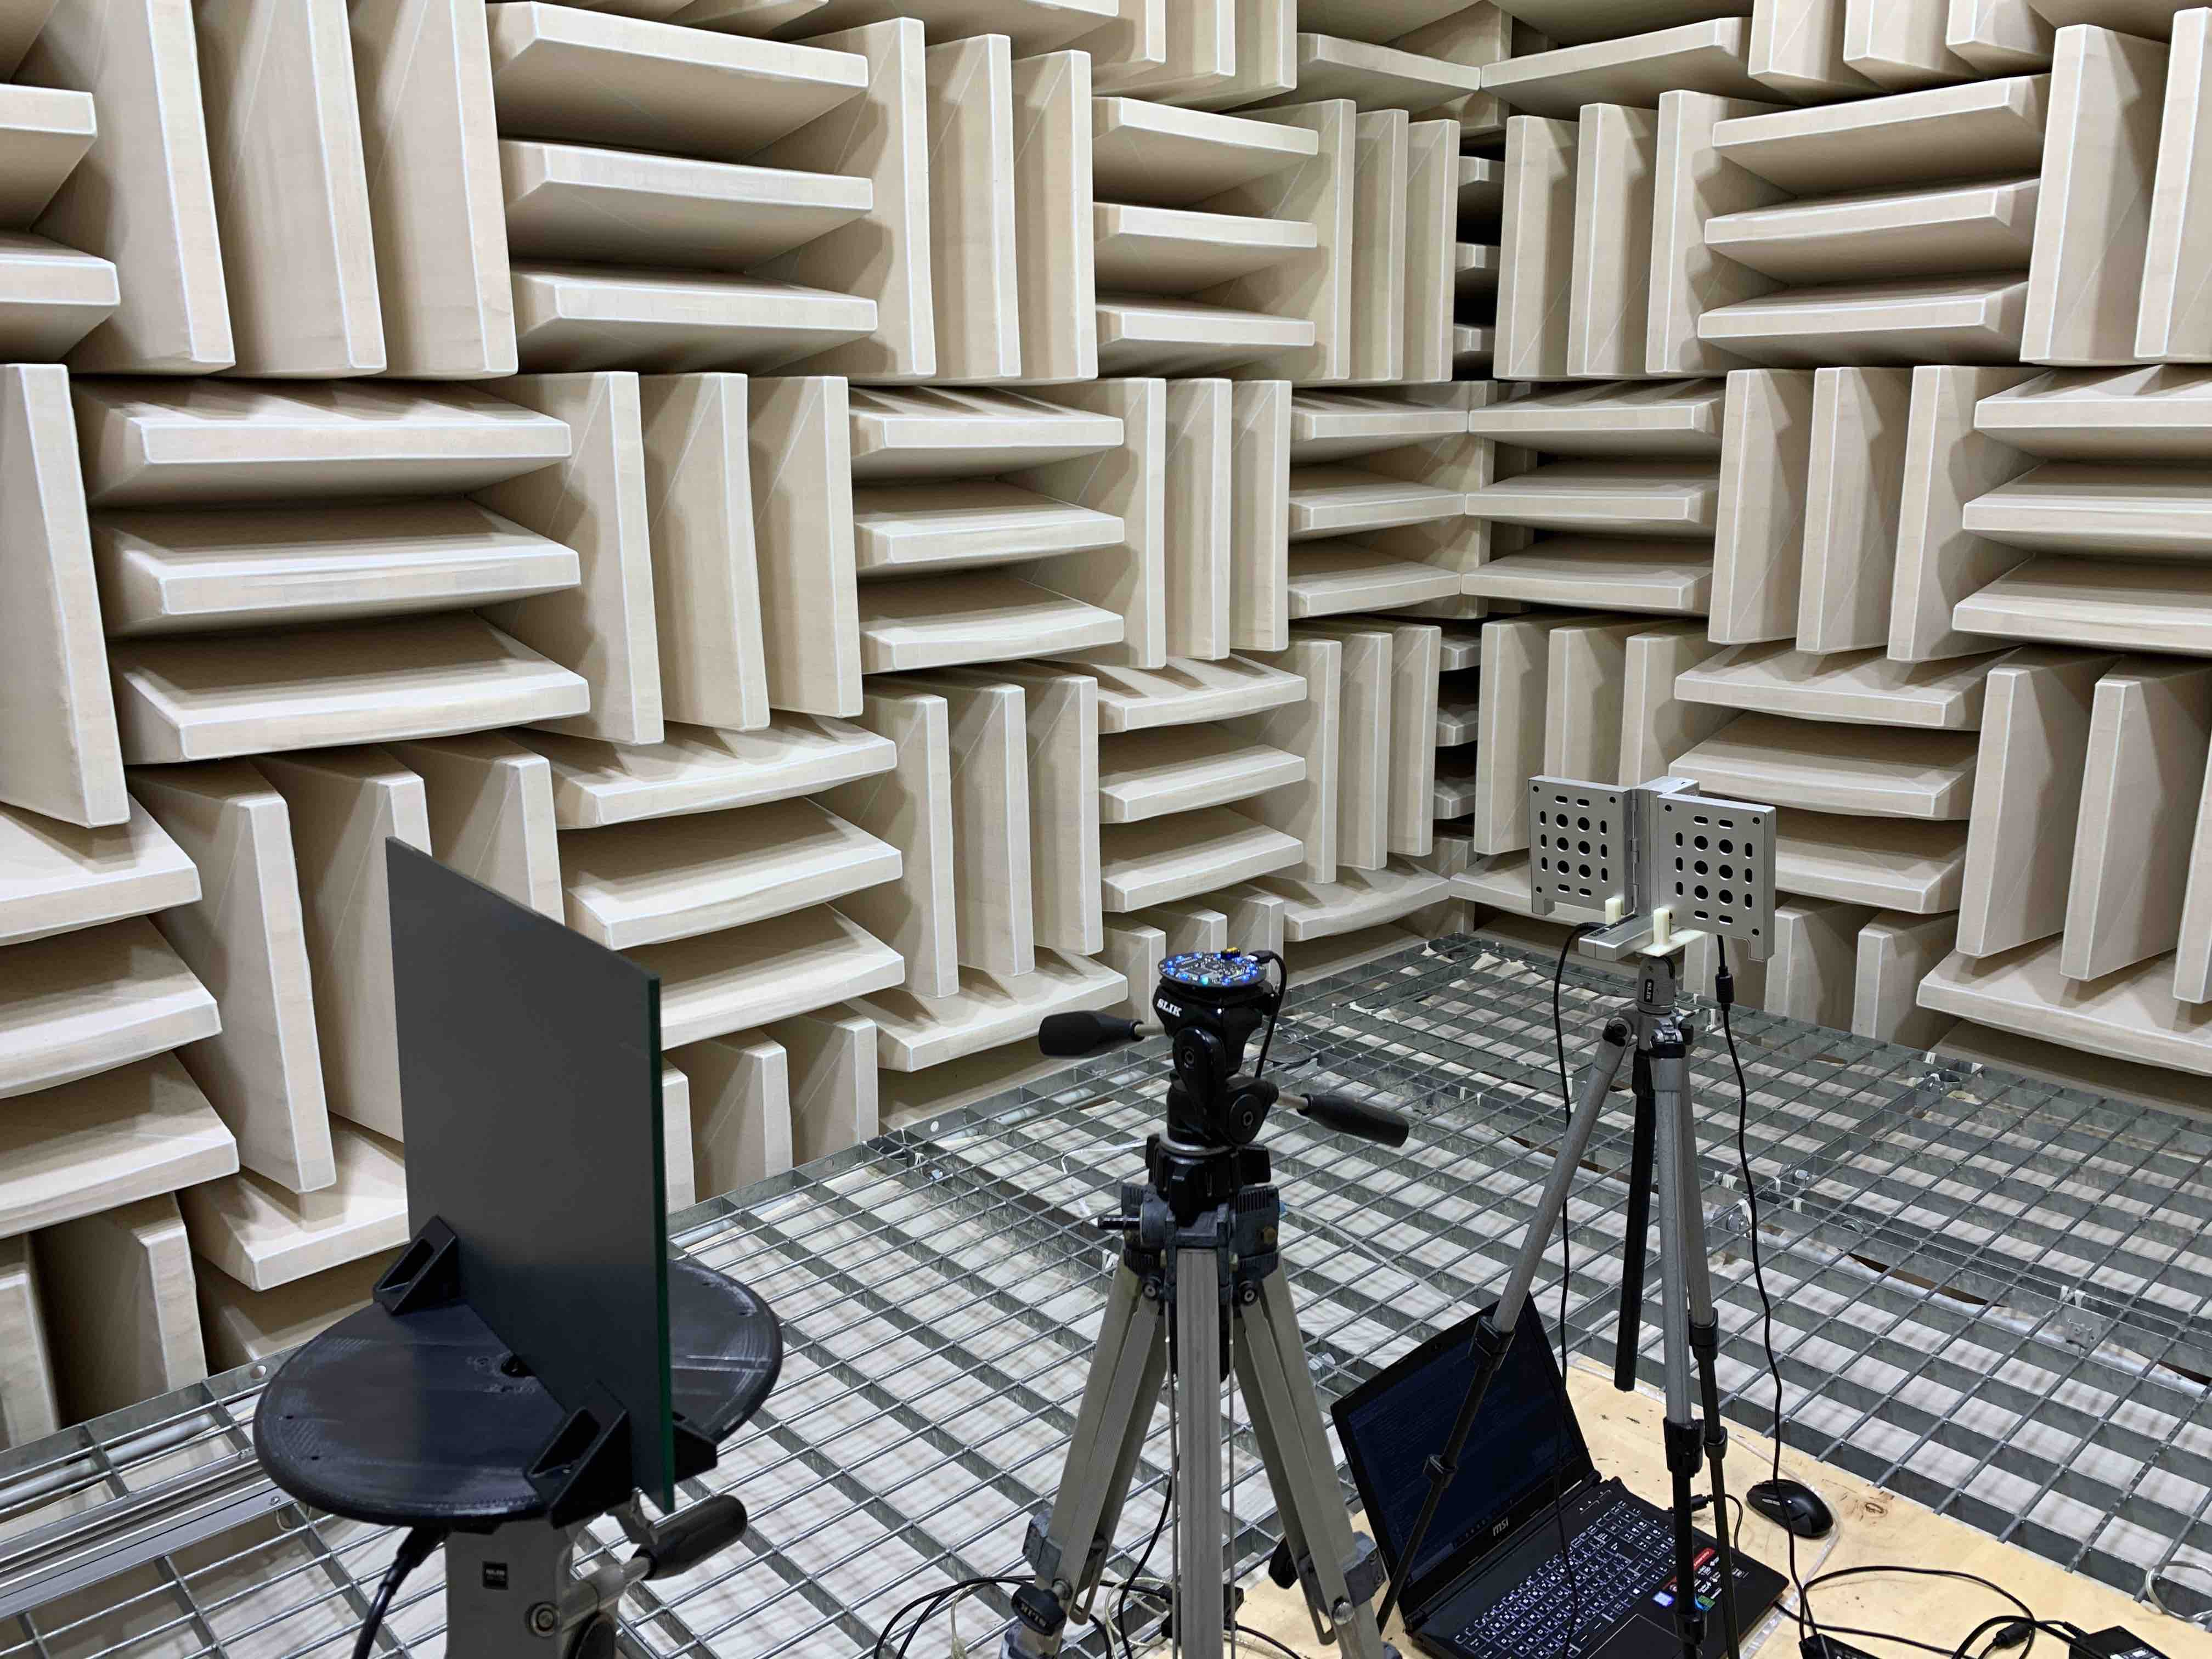
\includegraphics[width=0.6\linewidth]{images/3_exp_anechoic.jpg}  
  \end{center}
  \caption{Experiment for checking model}
  \label{fig:exp_env}
\end{figure}

\subsection{モデルを用いた場合の評価}
\label{sec:result_model}
\subsubsection{中、高域のエネルギーの変化}
(1)について、\figref{result1}はマイクで取得した音のフーリエ変換後の1000 [Hz]から2000 [Hz]のデータをプロットしたものである。フーリエ変換幅は全時間をフーリエ変換した。この結果の中でも$\psi=0, \psi=20$の値を描画したものである。
\figref{e-f}と比較しても、周波数領域において、考えたモデルのような結果を見ることはできなかった。



\subsubsection{エネルギー比と方位角の関係}
(2)について、\figref{result2}に示す.\figref{result1}のある周波数についての方位角と振幅の関係を見たものである。この結果より、モデル作成時の仮定としておいていた拡散反射と鏡面反射の割合によって、変化が見えるという予測に対して、1000[Hz], 2000[Hz]の比較と、\figref{result1}の結果も踏まえて考えると、周波数におけるモデルのときに考えた拡散反射、鏡面反射の割合の変化については考えることが難しいのでは無いかと考えた。しかし、一方で、ある周波数における方位角に対しての振幅の変化は連続的であり、かつモデルで考えていた形に似ている形をしている。そのため、この点より、方位角の角度と反射音にはある一定の関係性があることがわかる。

\subsubsection{方位角の推定}
(3)について、 \equref{d_n_fm_fh}に当てはめ、1000 [Hz], 2000[Hz]の値で割った結果を\figref{result3}に示す。結果としては、予測モデルとは違った変化の仕方をする。この原因としては、(1)の仮定について、これまでの結果より現状のデータでは当てはまらないことが大きいと考えられる。

\begin{figure}[ht]
  \begin{center}
  \vspace{1zh}
    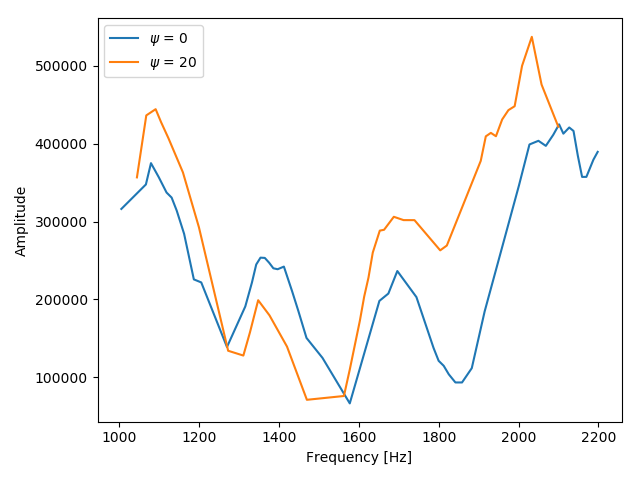
\includegraphics[width=0.5\linewidth]{images/3_amp_fre_heimen.png}   
  \end{center}
  \vspace{-2zh}
  \caption{elationship between energy (E) change with respect to frequency (f) and azimuth direction (N) when the sound source direction (S) and microphone direction (V)}
  \label{fig:result1}
\end{figure}

\begin{figure}[ht]
  \begin{center}
  \vspace{1zh}
    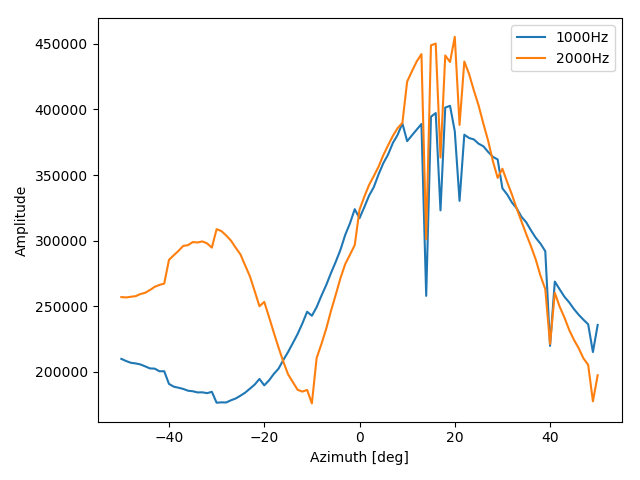
\includegraphics[width=0.5\linewidth]{images/3_amp_azi_heimen.png}   
  \end{center}
  \caption{Relation between energy ratio $D(\mathbf{N}|f_m, f_h)$ and azimuth angle $\mathbf{N}$ between mid and high frequencies at a point Q on the plane($f_m = 1000$, $f_h = 2000$)}
  \label{fig:result2}
\end{figure}

\begin{figure}[ht]  
  \begin{center}
  \vspace{1zh}
    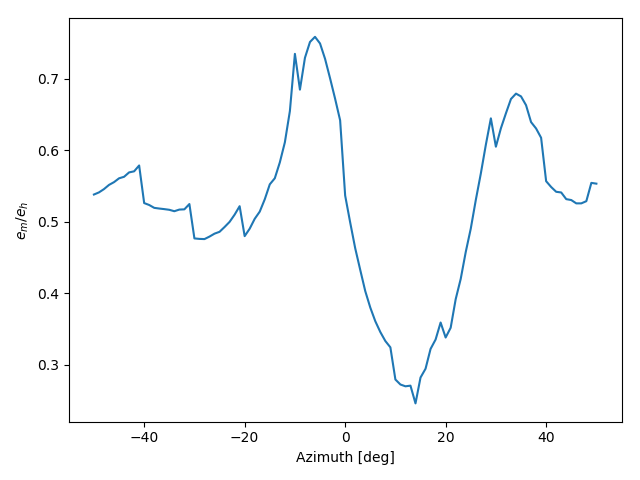
\includegraphics[width=0.5\linewidth]{images/3_d_n_heimen.png}   
  \end{center}
  \caption{Relation between energy ratio $D(\mathbf{N}|f_m, f_h)$ and azimuth angle $\mathbf{N}$ between mid and high frequencies at a point Q on the plane($f_m = 1000$, $f_h = 2000$)}
  \label{fig:result3}
\end{figure}

\clearpage

\subsection{モデル作成に関する考察}
\label{sec:model_dissucussion}
 結果として、(1)の周波数領域における振幅の関係がなかった。しかし、(2)方位角と振幅の関係は似たような関係を見ることができた。そのため、モデル自体を使うことはできないが、方位角と反射音には何かしらの連続的な関係があることがわかった。
 
 まずは、理論通りの結果にならない原因を考える。原因の一つは直接音の影響であると考える。今取得している音波は完全に反射音のみを取得しているのではなく、マイクには直接音と反射音の合成音が取得されている。さらに、もう一つが反射音の干渉である。この2点について、理論で考えたモデルでは、直接音は考えておらず、反射音はある1点の反射音のみを考えている。そのため、直接音、他の点での反射音が干渉した音をマイクで取得していることになる。この原因より、周波数領域での変化というのは干渉の影響を非常に受けやすいため、この結果になったと考えている。
 
 対策としては、2点考えられる。
 
 1点目はデータの改善である。方法は音声分離手法が考えられる。音声分離手法の中でも位置関係等が与えられるため、Beamformingを用いることが考えられるが、後の\secref{result_svr}で述べるが、結果としては、現在使用している4つのマイクロホンアレイでは空間分解能の精度が出ないため、難しいことがわかった。現状はDelay-Sum Beamforminを用いているが、MVDR Beamformingに代表される適応Beamforingについて今後検討をしていきたいと考えている。
 
 2点目はモデルの改善である。特に、不安があるのが、鏡面反射と拡散反射の周波数の変化による変化である。鏡面反射と拡散反射の割合について、参考にした論文は音響分野の論文で、壁等が対象物体であることが多い。そのため、ミクロな視点で考えた論文を再度探すか、実験等を繰り返していくことが必要だと感じた。
 
 \if 0
 
 この直接音と合成音の分離が必要だと考える。この分離する手法としては2つ考えられる。1点目はスピーカからの距離と物体までの距離がわかっている場合、直接音のみのデータを録音しておく。スピーカとマイクの出力に関して同期を取ることで音速よりマイクへの音の到達時間を計算し、音データの中でも直接音が取得される時点から直接音のみのデータを引く。2点目はBeamformerを用いた音域制限である。現在使用しているデータはマイクで取得されたデータをそのまま用いている。理論的には、ある一点Qからの音のみを知りたいため、Beamformingを用いることによって取得する方向を制限することができ、これにより直接音の影響を完全に消す事はできないが弱めることができると考えられる。

\fi

\newpage

\subsection{SVRを用いての評価}
\label{sec:result_svr}
\secref{result_model}より、方位角と反射音について関係があることがわかった。しかし、私自身では現状モデルを作成することができない。そこで、SVRの結果を参考にまたモデルについて考えていきたいと思う。
まず、SVRを用いての結果を\figref{result_svr_1}に示す。このとき、横軸は実際の対象面の角度、縦軸は推定した対象面の角度である。つまり、正解の値はオレンジの線のような直線がかけることがわかる。そのため、求める結果としては、このオレンジの線にどれだけ沿っているのかを評価する。

\begin{figure}[b]
    \centering
    \subfigure[Result using SVR anechoic data]{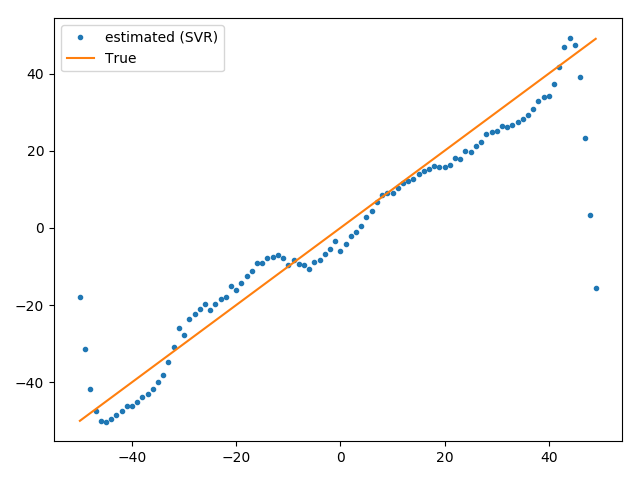
\includegraphics[width=0.48\linewidth]{images/3_anechoic_model_test_data.png}}
    \label{fig:result_svr_anechoic}
    \vspace{2zh}
    \subfigure[Result using SVR real
    data]{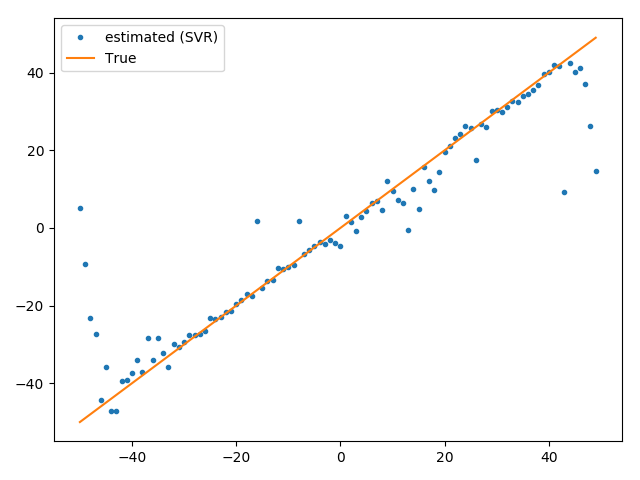
\includegraphics[width=0.48\linewidth]{images/3_real_model_test_data.png}}
    \label{fig:result_svr_real}
    \vspace{1zh}
    \caption{Result of Experiment based on SVR}
    \label{fig:result_svr_1}
\end{figure}

次に、無響室で作成したモデルを実環境での実験データでも予測ができるのかを検証した。その結果を\figref{result_svr_2}に示す。

このときのそれぞれの決定係数(Coefficient of determination, $\mathrm{R}^2$)と二乗平均平方誤差(Root Meen Squared Error, RMSE [deg])で評価した結果をTable. \ref{tab:result_svr_r2_rmse}に示す。

以上の結果より、SVRを用いることによって、5 [deg]以下の誤差で推定することができることがわかった。ここで、モデルベースでの結果について、考察をするために、現状の実験器具についてそれぞれ検証を行う。

使用した音の種類、周波数の範囲、スピーカについて、この組み合わせが正しかったのかを考察すべく、\secref{result_svr_sound_kind} $\sim$ \secref{result_svr_speaker}でそれぞれについて評価していく。

\begin{table}[ht]
\caption{Result of SVR}    
\vspace{1zh}
\centering
  \begin{tabular}{|l|p{6em}|p{6em}|} \hline
    Traing data/ Test data & $\mathrm{R}^2$ & RMSE [deg] \\ \hline\hline 
    Anechoic / Anechoic & 0.8 &  3.5 \\ \hline 
    Real / Real & 0.7 &  4.0 \\ \hline
    Anechoic / Real & 0.7 &  4.5 \\ \hline
  \end{tabular}
  \label{tab:result_svr_r2_rmse}
\end{table}


\begin{figure}[ht]
  \begin{center}
  \vspace{1zh}
    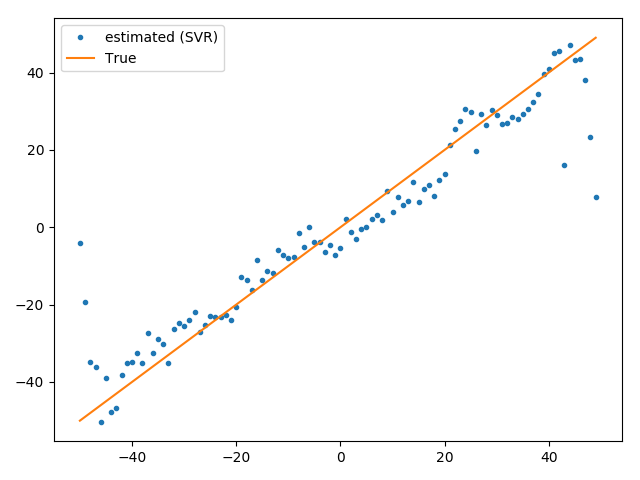
\includegraphics[width=0.48\linewidth]{images/3_anechoic_model_real_data.png}   
  \end{center}
  \caption{Result using SVR (traing data: anechoic data, test data: real data)}
  \label{fig:result_svr_2}
\end{figure}

\clearpage

\subsubsection{使う音の評価}
\label{sec:result_svr_sound_kind}
今回、音波として、TSP信号を用いている。このような、周波数成分を多く持ったデータを使うことが有効であるかどうかを確認する。

方法は、単一の高さの音を流した音の場合でも同様にデータを作成し、SVRをつかってモデル化したモデルを用いて、推定を行い、その二乗平均平方誤差を比較する。
この結果を\figref{result_sound_kind}に示す。

\figref{sound_kind_800} $\sim$ \figref{sound_kind_2000}より、単一の音を用いた場合は、SVRを用いても推定をすることはできていない。これは\figref{result2}からもわかるが、単一の音を切り取った場合その音には線形な関係を見ることができない。そのため、角度を推定することができなかったと考えられる。

そこで、800, 1000, 2000 [Hz]での3つのデータを連結することで、3つの周波数の情報をもつデータセットを作成した。そのデータセットを用いて同様にSVRのモデル作成し、テストデータで検証した結果を\figref{result_sound_kind_ver2}に示す。

\figref{result_sound_kind_ver2}のように、3つのデータを連結したデータを用いても認識はできなかった。この結果より、周波数領域のデータの重要性が理解できる。

そのため、TSP信号のように、周波数領域に関して、多くのデータを集めることができる信号を使うことはモデルベースで解く際にも有効であると考えられる。

\begin{figure}[b]
    \centering
    \subfigure[800Hz]{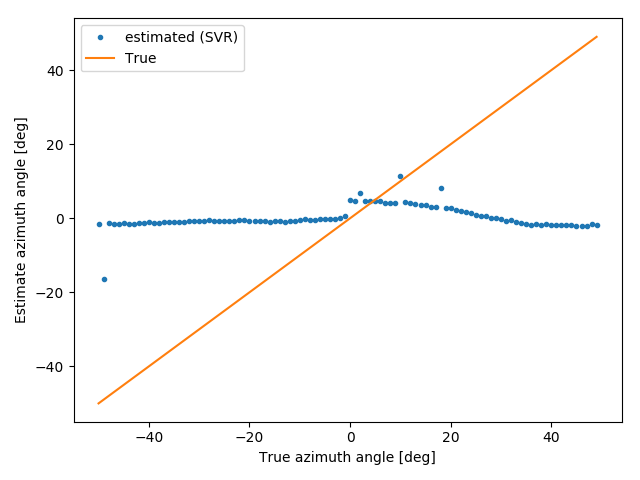
\includegraphics[width=0.45\linewidth]{images/3_svr_1015_PTo01_800.png}\label{fig:sound_kind_800}}
    \subfigure[1000Hz]{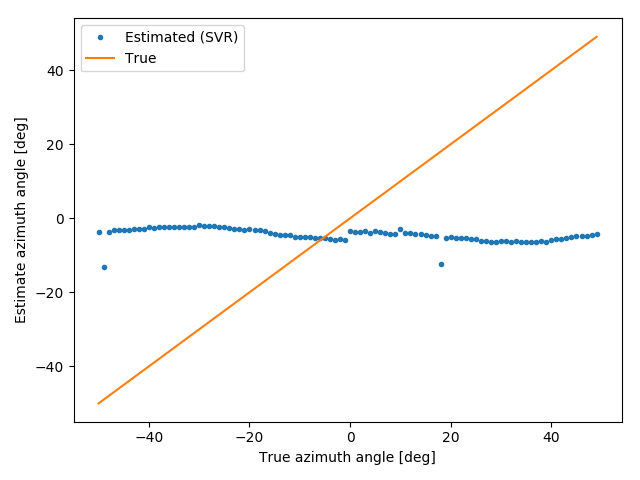
\includegraphics[width=0.45\linewidth]{images/3_svr_1015_PTo01_1000.png}\label{fig:sound_kind_1000}}
    \subfigure[2000Hz]{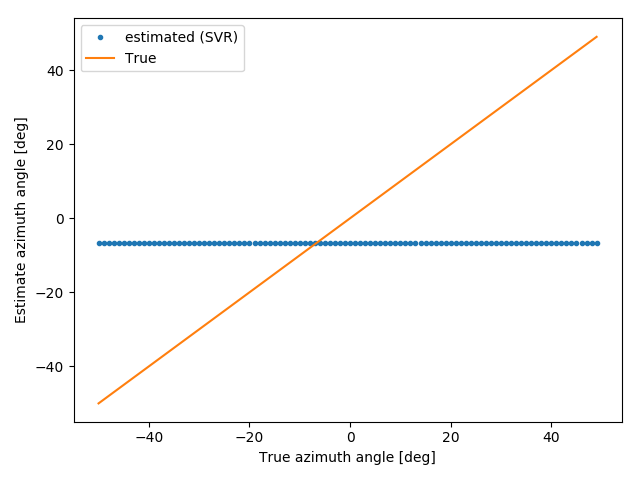
\includegraphics[width=0.45\linewidth]{images/3_svr_1015_PTo01_2000.png}\label{fig:sound_kind_2000}}
    \subfigure[Result using torn signal 800, 1000, 2000Hz]{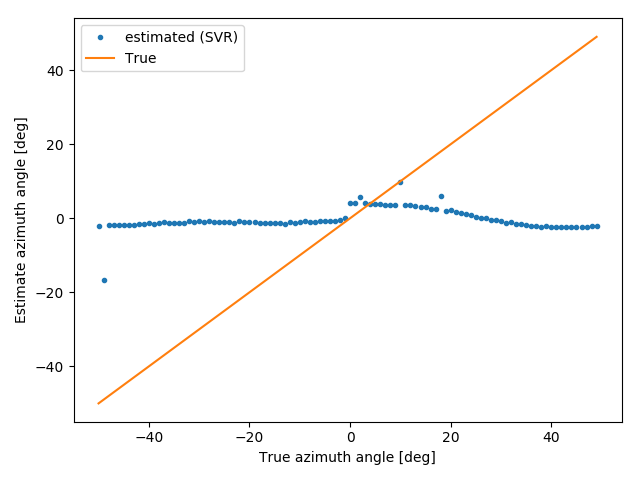
\includegraphics[width=0.45\linewidth]{images/3_svr_1015_PTo01.png}\label{fig:result_sound_kind_ver2}}
    \caption{Comparison of result about sound kinds}
    \label{fig:result_sound_kind}
\end{figure}

\if 0
\begin{figure}[ht]
  \begin{center}
  \vspace{1zh}
    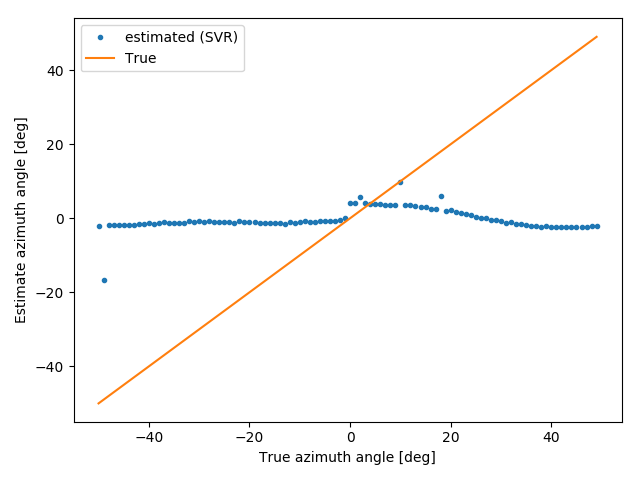
\includegraphics[width=0.5\linewidth]{images/3_svr_1015_PTo01.png}   
  \end{center}
  \caption{Result using torn signal (800, 1000, 2000[Hz])}
  \label{fig:result_sound_kind_ver2}
\end{figure}
\fi

\clearpage

\subsubsection{使う周波数の範囲の評価}
\label{sec:result_svr_freq_renge}
今回、使用する音の周波数として、音の反射の特性の変化を用いるために1000 [Hz]から2000[Hz]の音波を使用した。今回、このような音を用いることが有効であるかどうかを確認する。

方法として、1000[Hz]から1000[Hz]おきにこれまでと同様の方式でデータセットを作成し、それぞれの決定係数、二乗平均平方誤差を比較する。結果をそれぞれ\figref{result_freq_renge_2}, \tabref{result_freq_range_r2_rmse}に示す。

\tabref{result_freq_range_r2_rmse}、\figref{result_freq_renge_2}より、0 $\sim$ 1000 [Hz]と6000 [Hz]以上の音のデータに関して、著しく結果が悪いことがわかる。この原因としては、2点考えられる。1点目はスピーカの出力の周波数応答、2点目はマイクの感度の周波数応答である。スピーカの周波数応答に関して、使用しているスピーカの周波数応答は0 $\sim$ 1000 [Hz]において、出力が低くなっている。この原因により、0 $\sim$ 1000 [Hz]において、音が安定しないため、0 $\sim$ 1000 [Hz]において、SVRの推定結果が悪くなったと考えられる。

次に、マイクの感度に関して、5000[Hz]以上においてマイクの感度が上がっている。そのため、スピーカのときと同様に、5000[Hz]で徐々に精度が下がり、6000[Hz]を超えるとRMSE 10 [deg]になり、\figref{result_freq_renge_2}で見た際のずれも明らかに大きくなっていると考えられる。

最後に、2000[Hz] $\sim$ 4000[Hz]の音が使いやすく、その中でも\figref{result_freq_renge_2}では、2000 $\sim$ 3000 [Hz]がきれいに見え、\tabref{result_freq_range_r2_rmse}では、RMSEが一番小さいのは3000 $\sim$ 4000 [Hz]になる理由はこれらのスピーカの出力とマイクの感度の最大出力と最低出力のちょうど中間程度であるため、安定しているためであると考えられる。

これらの結果より、今回検証したかった、1000 $\sim$ 2000 [Hz]における反射特性の変化が重要であるという仮定について、本実験では検証できなかった。本実験では、マイクとスピーカの感度が安定する点であれば、モデルを作成することができるとわかった。

今後、モデルベースで解く際にはスピーカから出す音に関しては、スピーカとマイクの許容範囲ギリギリではなく、余裕を持った音の高さを用いることが有効であることがわかった。しかし、音の反射特性の変化を用いることが有効であるか否かについては本実験では、検証することができなかった。今後、違った方法で検証していこうと考えている。

\begin{figure}[p]
  \centering  
  \vspace{-7zh}
    \subfigure[$0$-$1000$Hz]{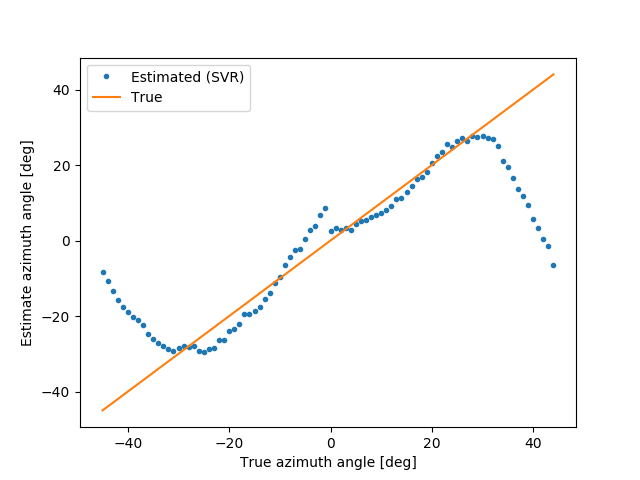
\includegraphics[width=0.4\linewidth]{images/3_svr__191015_PTs01_freq_0.png}
     \label{fig:freq_range_0}}
    \subfigure[$1000$-$2000$Hz]{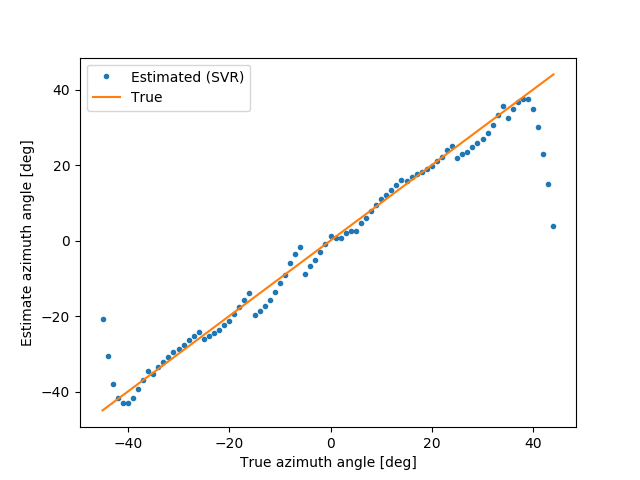
\includegraphics[width=0.4\linewidth]{images/3_svr__191015_PTs01_freq_1000.png}
     \label{fig:freq_range_1000}}
    \subfigure[$2000$-$3000$Hz]{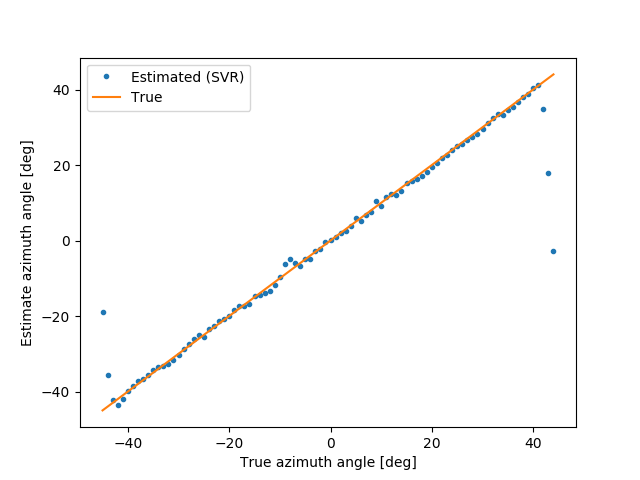
\includegraphics[width=0.4\linewidth]{images/3_svr__191015_PTs01_freq_2000.png}
     \label{fig:freq_range_2000}} 
    \subfigure[$3000$-$4000$Hz]{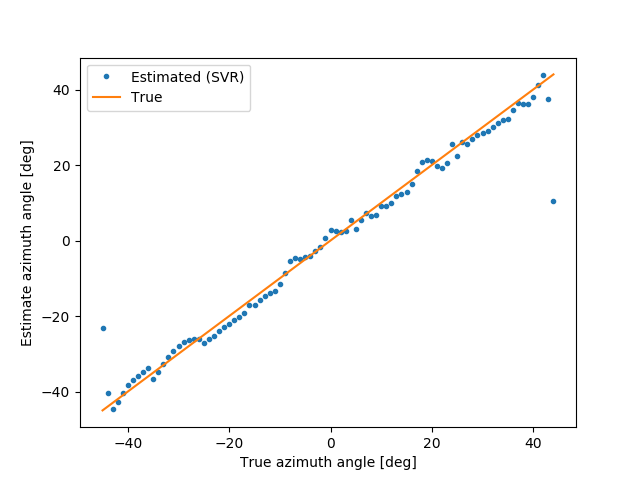
\includegraphics[width=0.4\linewidth]{images/3_svr__191015_PTs01_freq_3000.png}
     \label{fig:freq_range_3000}}
    \subfigure[$4000$-$5000$Hz]{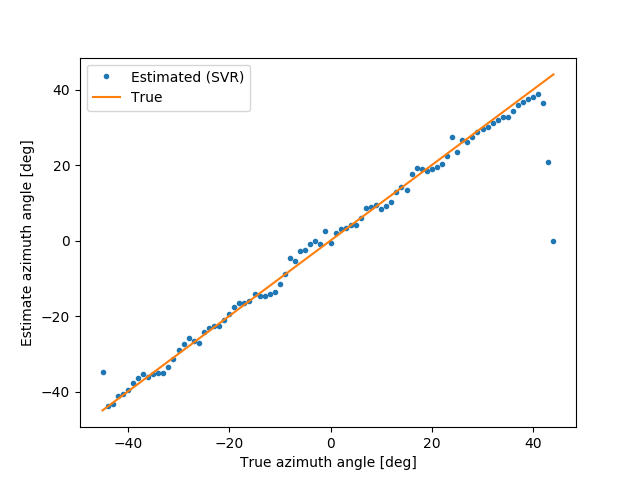
\includegraphics[width=0.4\linewidth]{images/3_svr__191015_PTs01_freq_4000.png}
     \label{fig:freq_range_4000}} 
    \subfigure[$5000$-$6000$Hz]{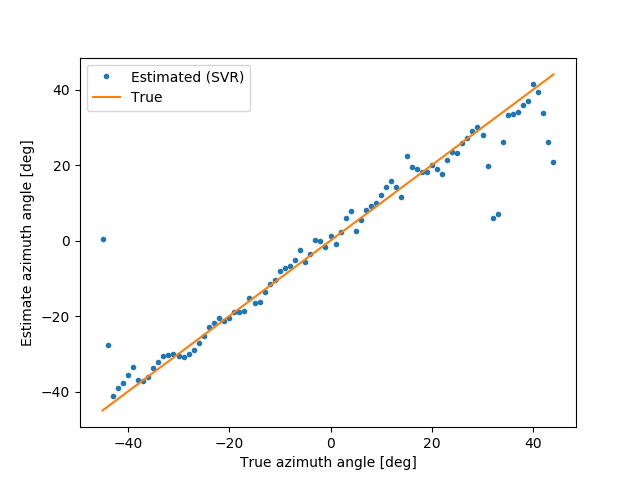
\includegraphics[width=0.4\linewidth]{images/3_svr__191015_PTs01_freq_5000.png}
     \label{fig:freq_range_5000}}  
     \subfigure[$6000$-$7000$Hz]{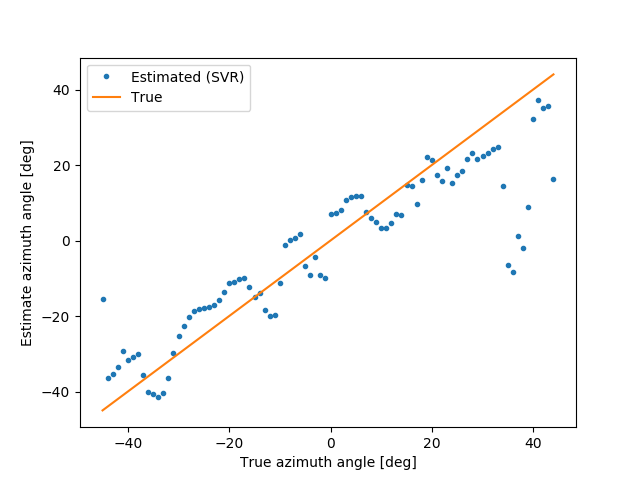
\includegraphics[width=0.4\linewidth]{images/3_svr__191015_PTs01_freq_6000.png}
     \label{fig:freq_range_6000}}     \subfigure[$7000$-$8000$Hz]{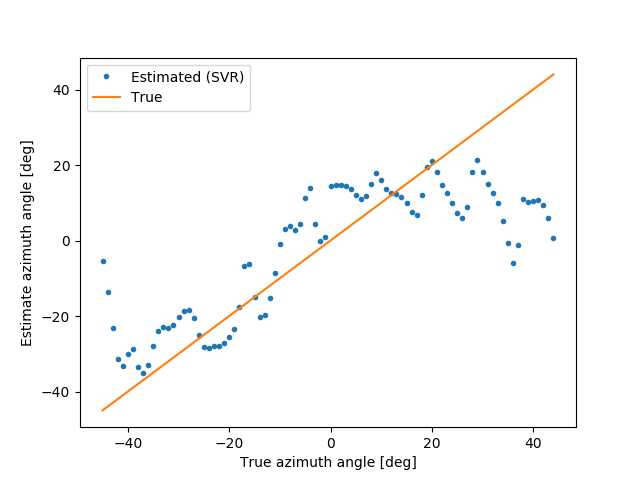
\includegraphics[width=0.4\linewidth]{images/3_svr__191015_PTs01_freq_7000.png}
     \label{fig:freq_range_7000}}    
     \caption{Comparison of frequency range based on case that I create models individually}
    \label{fig:result_freq_renge_2}
\end{figure}

\begin{table}[ht]
\caption{Comparison of $\mathrm{R}^2$, RMSE by change of freequency range}    
\vspace{1zh}
\centering
  \begin{tabular}{r||p{6em}|p{6em}} \hline
    Frequency Range [Hz] & $\mathrm{R}^2$ & RMSE [deg] \\ \hline\hline 
    0 $\sim$ 1000 & 0.692 &  14.218 \\ \hline 
    1000 $\sim$ 2000 & 0.934 &  6.482 \\ \hline
    2000 $\sim$ 3000 & 0.939 &  6.437 \\ \hline
    3000 $\sim$ 4000 & 0.969 &  4.469 \\ \hline
    4000 $\sim$ 5000 & 0.955 &  5.826 \\ \hline
    5000 $\sim$ 6000 & 0.915 &  9.780 \\ \hline
    6000 $\sim$ 7000 & 0.786 &  11.067 \\ \hline
    7000 $\sim$ 7000 & 0.624 &  15.971 \\ \hline
  \end{tabular}
  \label{tab:result_freq_range_r2_rmse}
\end{table}

\clearpage

\subsubsection{使うスピーカの評価}
\label{sec:result_svr_speaker}
今回の実験では、平面波のスピーカを用いている。しかし、これが球面波スピーカの場合ではどうなるのかを確認する。

方法は球面波スピーカで発した音のデータを同様に作成したものでSVRをもちいてモデルを作成した。このときのスピーカはONKYO社のパワードスピーカシステム GX-D90を用いている。GX-D90について、使用した物の写真を\figref{exp_spherical_wave}に示す。今回、本来はステレオスピーカとして、2対でつかうものであるが、\figref{exp_spherical_wave}のように、片方のみでしようした。理由としては、二つの方向から同時に音がなることによる干渉を避けるためである。
この実験における結果を\figref{result_speaker_kinds}に示す

この結果は\figref{result_speaker_kinds}となった。このときのRMSEは24.961 [deg]であり、球面波スピーカを用いた場合、これまでの平面波スピーカを使用した場合と比べて、SVRでの推定ができなくなっていることがわかる。以上の結果より、スピーカとして、平面波スピーカを用いたことはモデルベースで解く場合にも有効な手段であると考えられる。

\begin{figure}[ht]
    \centering
    \subfigure[GX-D90 ONKYO Inc.]{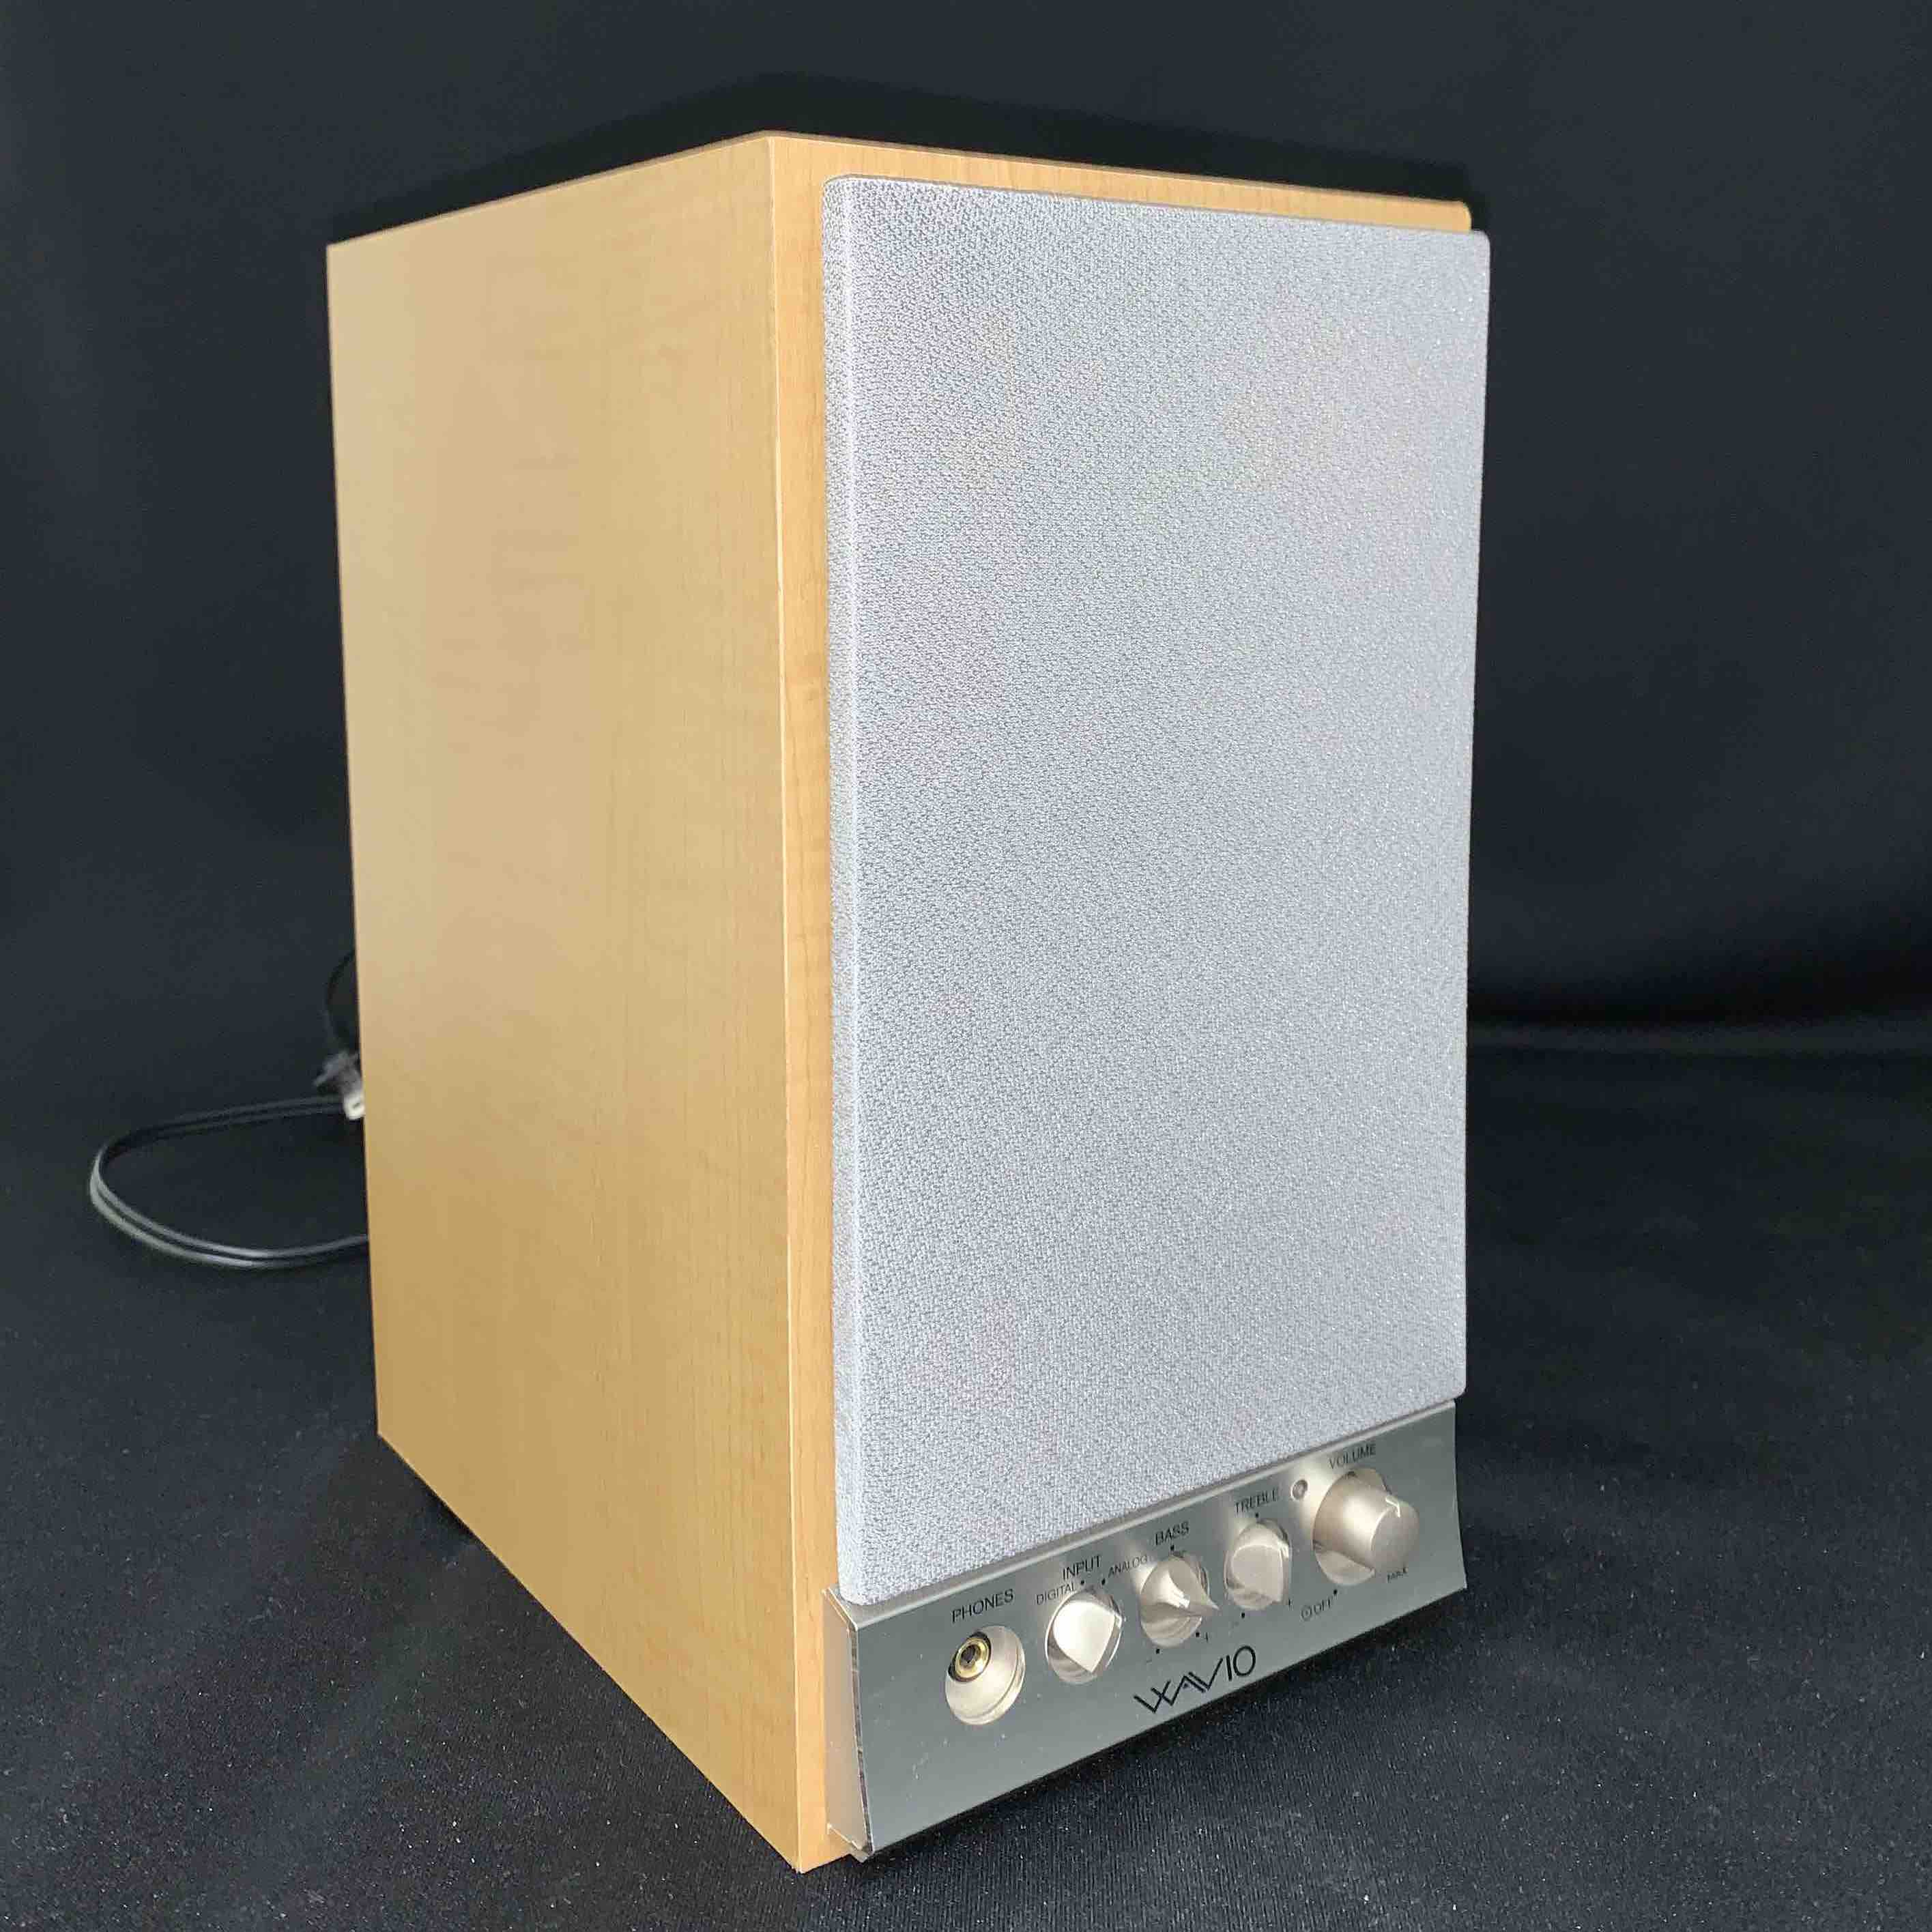
\includegraphics[width=0.4\linewidth]{images/3_specular_speaker.jpg}\label{fig:exp_spherical_wave}}
    \subfigure[Result of the data by spherical wave]{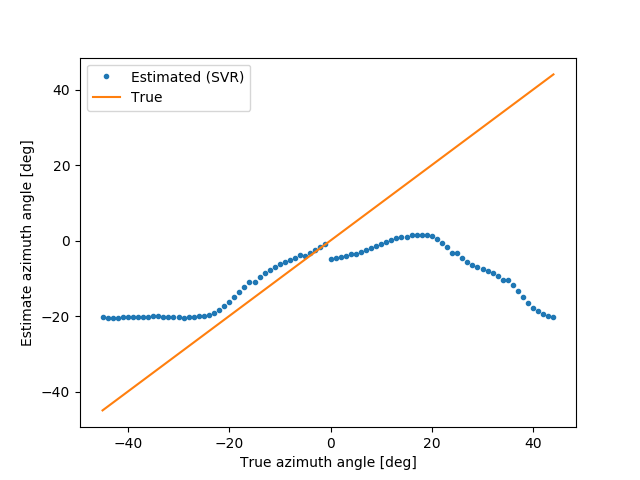
\includegraphics[width=0.5\linewidth]{images/3_svr__191015_STs01.png}\label{fig:result_speaker_kinds}}
    \caption{Experiment for speaker speculat speaker}
    \label{fig:beam_check}
\end{figure}

\clearpage

\subsection{SVRを用いた場合の考察}
SVRを用いた場合、物体平面の面の方向を誤差5 [deg]以下で推定することができた。このように推定できた理由としては、物体平面の方位角とある周波数でのパワースペクトルの様子には連続的な関係があった。この連続的な関係については、\figref{result2}にてすでに示している。このような変化の特徴を使うことでSVRでは推定モデルを作成することができたと考えている。

しかし、\secref{model_dissucussion}でも述べたが、このような変化はモデルベースで解く際には考えていた変化とは違う。
この原因として、直接音や他の点の反射音の影響が考えられ、対策として、音声分離手法のBeamformingを考えた。そこで、Delay-Sum Beamforming を用いて、対象物体の中心から反射してきた音を分離した。この分離音を用いて、SVRのモデルを作成し、推定した結果を\figref{exp_beam_check}で示す。

\figref{exp_beam_check}より、精度はBeamforming前よりも低下した。この理由としては、2点あると考えている。1点目はBeamforingの精度が悪い。[参考文献]より、4個のマイクアレイではほとんど分離が不可能であることがわかる。このように、分離の精度が悪いと考えられる。
2点目は、物体形状の影響が大きいという点である。物体形状の情報をわざと消しているBeamformingを用いることでその情報が落ち、精度が落ちたと考えられる。

\if 0
\begin{figure}[ht]
    \centering
    \subfigure[Beamforming result]{
\includegraphics[width=55mm]{images/fig_sample.png}\label{fig:beam_check_intensity}}
    \subfigure[SVR result using beamforming data]{
\includegraphics[width=55mm]{images/fig_sample.png}\label{fig:beam_check_svr}}
    \caption{Result of beamforming}
    \label{fig:beam_check}
\end{figure}
\fi

\begin{figure}[ht]
  \begin{center}
  \vspace{1zh}
    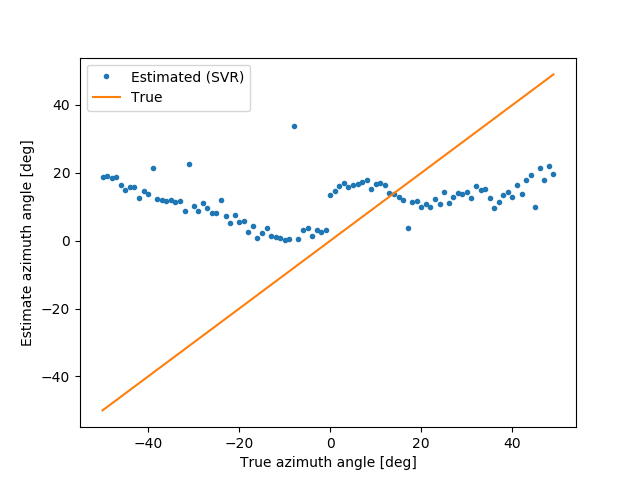
\includegraphics[width=0.6\linewidth]{images/3_svr_191015_PTs01_beam.png}   
  \end{center}
  \caption{SVR result using beamforming data}
  \label{fig:exp_beam_check}
\end{figure}

このような結果より、3点の疑問点もできた。
\begin{itemize}
    \item 材質による影響はどの程度あるのか?
    \item 物体の大きさを小さくしても認識可能か?
    \item 複数面でも認識可能か?
\end{itemize}
上記の3点について、次の節で検証していく。

また、SVRにおいて、どの周波数に関係があるのか?、どのような関係が見えるかを調べるために、主成分分析とパラメトリック固有空間法を用いて、検証を行った。その検証について、\secref{PCA}で行う。

\if 0
\begin{figure}[ht]
  \begin{center}
  \vspace{1zh}
    
\includegraphics[width=0.5\linewidth]{images/fig_sample.png}   
  \end{center}
  \caption{Relationship of intensity and azimuth angle in 1000 [Hz]}
  \label{fig:relation_intensity_azimuth}
\end{figure}
\fi


\subsubsection{サポートベクターの解析}
\label{sec:PCA}
まず、主成分分析を用いて、第一、第二、第三主成分の周波数における固有値の変化を無響室でのデータ、現実環境でのデータそれぞれで比較する。
結果を\figref{pca_check}に示す。

このように、両者は似たような変化をしていることがわかる。この変化にサポートベクターは着目しているため、無響室でのモデルが実環境のデータに当てはめることができたと考えられる。

次に、パラメトリック固有空間法をもちいて解析を行う。この手法を用いるために、第一主成分から第三主成分までの主成分を3軸として3次元プロットを行う。このような方法は、実際のデータに今回のような物理的な変化がある際に用いることで、3次元プロットした際にある規則的な動きをすることがあり、そこからモデル化の道筋を立てることができる。
今回の場合、角度が-50から50で回転しているため、回転のような連続的な動きが見れることが望ましい。
無響室データ、実環境データそれぞれの結果を\figref{pes_check}に示し、このときの、主成分分析の寄与率をTable. \ref{tab:pes_contri}に示す。

\begin{figure}[ht]
    \centering
    \subfigure[PCA anechoic data]{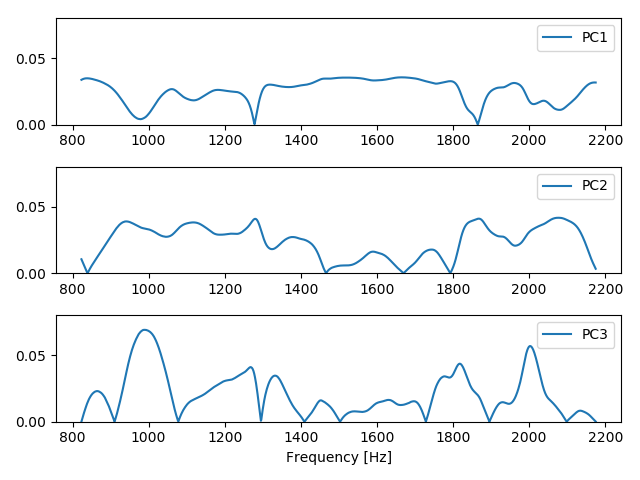
\includegraphics[width=55mm]{images/3_pca_pc1_pc3_anechoic_ve2.png}}
    \label{fig:pca_check_anechoic}
    \subfigure[PCA real data]{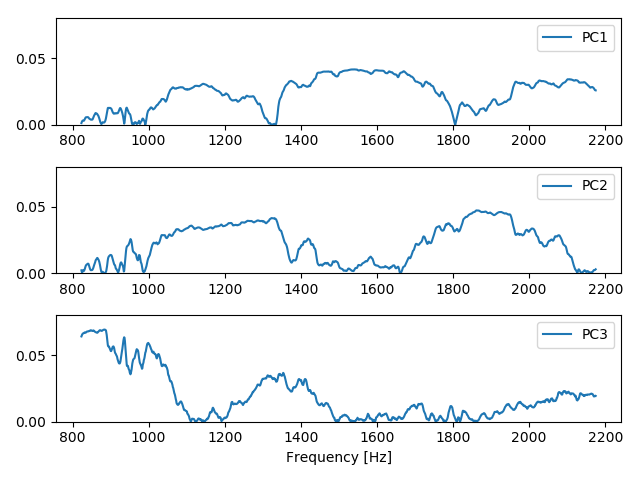
\includegraphics[width=55mm]{images/3_pca_pc1_pc3_real_ver2.png}}
    \label{fig:pca_check_real}
    \caption{Result of PCA}
    \label{fig:pca_check}
\end{figure}

\begin{figure}[ht]
    \centering
    \subfigure[Parametric eigen space method of anechoic data]{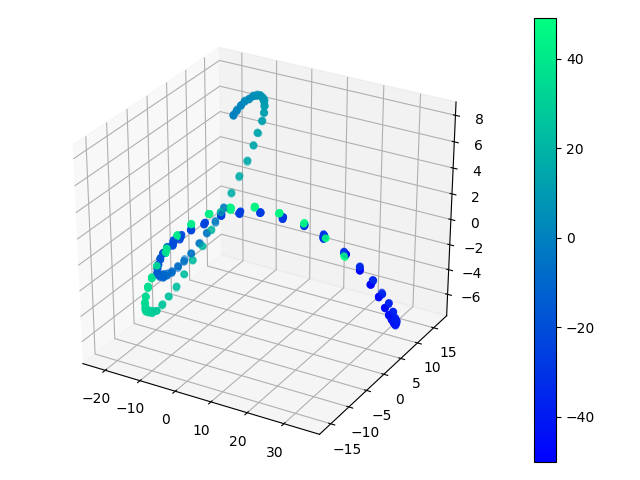
\includegraphics[width=55mm]{images/3_pca_1025_anechoic.png}}
    \label{fig:pes_check_anechoic}
    \subfigure[Parametric eigen space method of real data]{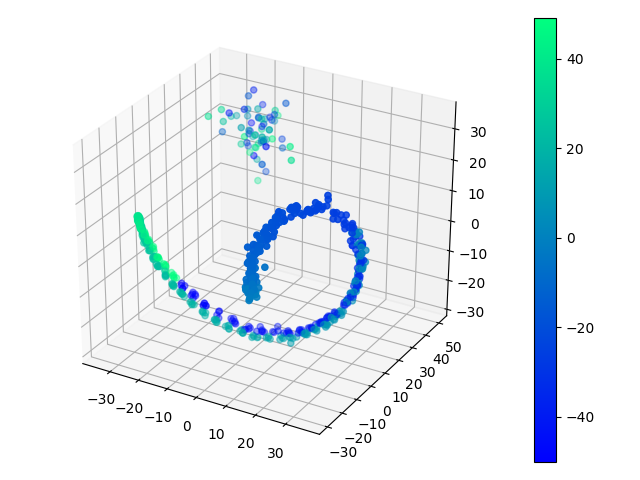
\includegraphics[width=55mm]{images/3_pca_1205_real_loading.png}}
    \label{fig:pes_check_real}
    \caption{Parametric eigen space method}
    \label{fig:pes_check}
\end{figure}

\begin{table}[ht]
    \centering
    \caption{Contribution rate}
    \vspace{1zh}
    \begin{tabular}{|c||p{4em}|p{4em}|} \hline
        PC & Anechoic & Real \\ \hline\hline
        PC1 & 0.73 & 0.52 \\ \hline
        PC2 & 0.18 & 0.13 \\ \hline
        PC3 & 0.03 & 0.05 \\ \hline
        SUM & 0.91 & 0.68 \\ \hline
    \end{tabular}
    \label{tab:pes_contri}
\end{table}

\clearpage

以上の結果より、確かに取得した音データの中には方位角による連続的な関係があることはわかった。さらに、動きもなめらかに円を描くような結果を出力している。このような点より、方位角と反射音の周波数領域の大きさには連続的な関係が見ることはできる。このため、サポートベクターによる回帰が可能であったと考えられる。

しかし、この図よりモデルを作成するのに必要な情報を取得することはできず、モデルベースで解くことは現状難しい。今回は可聴域の音波を最初の理由より用いていたが、今後は超音波を使用することを考えたい。理由としては、超音波は直進性が強いため可聴域よりも光の特性に似ている。こういった理由より、モデルベースで解く場合には超音波を用いることが良いと考えている。

\clearpage
\newpage
